\documentclass[a4paper,12pt]{article}
%\usepackage[utf8x]{inputenc}
\usepackage[utf8]{inputenc}
%\usepackage{lipsum}
\usepackage{amsmath,amsthm,mathrsfs}
\usepackage[english]{babel}
\usepackage{textcomp}
%\usepackage[T1]{fontenc}
\usepackage{graphicx,wrapfig}
\usepackage{amssymb}

\newcommand\norm[1]{\left\lVert#1\right\rVert}
\usepackage{calc}
\usepackage{rotating}
\usepackage[usenames,dvipsnames]{color}
\usepackage{fancyhdr}
%\usepackage{subfigure}
\usepackage{hyperref}
\usepackage{longtable}
\usepackage{svg}
\usepackage{float}
\usepackage{rotating}
\usepackage[usenames,dvipsnames]{color}
\usepackage{fancyhdr}
%\usepackage{subfigure} 
\usepackage[english]{babel}
\usepackage[backend=bibtex,
style=numeric,
bibencoding=ascii,
sorting=none
%style=alphabetic
%style=reading
]{biblatex}
\usepackage{hyperref}
\addbibresource{btp_final}
\usepackage[a4paper, margin=1.5in]{geometry}
\usepackage{pifont}
\usepackage{xcolor}
\usepackage{dirtytalk}
\hypersetup{
    colorlinks,
    linkcolor={red!50!black},
    citecolor={blue!50!black},
    urlcolor={blue!80!black}
}
\graphicspath{{images/}}
%\usepackage{times}
%\usepackage[scaled=0.8]{beramono}
 \renewcommand{\familydefault}{\rmdefault}

\begin{document}

\begin{titlepage}
\pagenumbering{gobble}
\begin{center}

 
%	\noindent\rule[0.5ex]{\linewidth}{4pt}
%  

  \vskip.1in
  \textbf{\Large Robust Controller Design Using \textbf{$H_{\infty}$}-Loop Shaping Approach}  \vskip.7in
  \vskip.7in
%\noindent\rule[0.5ex]{\linewidth}{4pt}
	\begin{center}\textit{\small{In partial fulfillment of the requirements}} \\
	\textit{\small{for the degree of}}
	\vskip.5in
	\large{\normalsize BACHELOR OF TECHNOLOGY}
	\vskip.3in
	\textit{by}
	\vskip.3in
	
	\textbf{\normalsize AYUSH PANDEY}\\
	\end{center}
\end{center}
%\vskip1.3in
%\begin{minipage}[t]{7cm}
%\flushleft
%\textsc{Author:}
%%
%Ayush Pandey \\12IE32001\\ IIT Kharagpur \\
%\end{minipage}
%\hfill
%\begin{minipage}[t]{7cm}
%\flushright
%\textsc{Supervisor:}
%
%Dr. Sourav Patra \\IIT Kharagpur
%\end{minipage}
%\vskip1.2in
\vskip.9in
\vskip.9in
\vskip.3in

\begin{center}

\includegraphics[scale=0.18]{logo}
\vskip.1in
\textbf{Department of Electrical Engineering}
\\
Indian Institute of Technology, Kharagpur
\\
West Bengal, INDIA 721302\\
May 2016

\end{center}
\end{titlepage}

\begin{wrapfigure}[1]{l}{0.001\textwidth}

\includegraphics[width=0.15\textwidth]{logo}
\end{wrapfigure}

\setlength{\parindent}{85pt}

 \large{Department of Electrical Engineering\\
} \-\hspace{3cm}\normalsize{Indian Institute of Technology, Kharagpur}
\\
 \-\hspace{3cm}West Bengal, INDIA 721302\\
 \-\hspace{3cm}November 2015\\ \\
\rule[2pt]{1.1\linewidth}{1pt}
\vskip.9in
\begin{center} \Large{\textbf{Certificate}} \end{center}
\vskip.4in
{\setlength{\parindent}{0cm}This is to certify that the report entitled \textbf{Robust Controller Design Using
$H_{\infty}$ Loop Shaping Approach}, submitted by \textbf{Ayush Pandey}, an undergraduate student, in the \textit{Department of Electrical Engineering, Indian Institute of Technology,
Kharagpur, India,} for the award of the degree of Bachelor of Technology, is a record of
the work carried out by him under our supervision and guidance. Neither this report nor any part of it has been submitted for any degree or academic award elsewhere.}
\vskip.9in
\vskip.9in
\parindent=0em
\begin{minipage}[p]{10cm}
\begin{flushleft}
\textbf{Dr. Sourav Patra}
\\Assistant Professor,\\
Department of Electrical Engineering,\\ Indian Institute of Technology,
Kharagpur,\\ INDIA 721302
\end{flushleft}
\end{minipage}

\vskip.9in
\vskip.9in
\vskip.9in
\vskip.9in

\vskip.9in
\vskip.9in
\vskip.9in
\vskip.9in
\vskip.9in
\vskip.9in

\begin{flushleft}

\Huge \textbf{Acknowledgements}
\end{flushleft}
\vskip.6in
I would like to take this opportunity to thank and acknowledge the help and support of the people who have been directly or otherwise involved with the work presented in thesis.\\
I am humbled by the support of my advisor Professor Sourav Patra. It his only because of his guidance and continuous support that I have been able to work persisently on this project.\\
I also wish to thank the Professors who have evaluated my project progress from time to time. The reviews and the evaluation certainly motivated me to work even harder on the project. I also owe my gratitude to Ganesh who helped me during the very beginning of this project by properly presenting a layout for me to go ahead with this project.\\
Also, I can't imagine having survived through the tough times without the support of fellow classmates and friends. Finally, I would like to thank my family. Without their love and support, none of this would have been possible.
\vskip.6in
\begin{flushleft}
Ayush Pandey\\
IIT Kharagpur

\end{flushleft}
\newpage
\pagenumbering{arabic}
{\hypersetup{linkcolor=blue}
\tableofcontents
}
\newpage
\section{Introduction}
Robustness of a system is defined by its ability to be insensitive to parameter variations and unwanted exogenous signals. For a control system, these variations could either be plant disturbances and parameter variations within the plant or these could be due to the sensor noises in measurement. Also, at times it is not possible to model the system dynamics accurately. These unmodeled plant dynamics may also affect the system in undersired manner.(See the block diagram in Figure(\ref{simple_siso})).
\begin{figure}[H]

			  \centering
			  \includesvg[width=1.0\textwidth]{block2}
%			  \def\svgscale{5.5}
%			  \tiny{
%			  \input{ulft.pdf_tex}}
			  \caption{Control System Block Diagram\\ \footnotesize n-Sensor Noise, r-Reference Input, y-Outpt, P-Plant, C-Controller, F-Feedback, di-Input Disturbance, do-Output Disturbance, e-Error, u-Control Input}
			 \label{simple}
		\end{figure}	
	 Hence, the aim of a control engineer is to design a controller in such a way that it deals with these uncertainities. The classical control theories, though, provide good performance for SISO systems but they are, in general, not replicable to multivariable systems. To overcome these
difficulties and to achieve a robust performance in MIMO systems several successful design methods have been developed in the past three decades. Among them, the $H_{\infty}$ control is a popular and effective robust control design technique.  \\
The theory of robust control was first proposed in the late 1970s and early 1980s and since then there has been a huge effort in various methods to achieve specified performance of a system robustly. The most widespread and important of these methods is the $H_{\infty}$ loop-shaping technique which was proposed by McFarlane and Glover of Cambridge University. The $H_{\infty}$ loop-shaping technique combines classical loop-shaping concepts with the $H_{\infty}$ controller design techniques.  \\
For application of a robust controller to a particular application the constraints of the system need to be modeled as well and the controller design has to be changed accordingly. This project aims to study in detail the $H_{\infty}$ loop-shaping robust controller design technique and then model a mobile robot system in such a way that a robust controller for the mobile robot's locomotion is designed. Some challenges that might be faced in this process are those concerning the complexity of the very theory of  $H_{\infty}$	 loop-shaping technique. Moreover, designing the controller for a mobile robot would be faced with many challenges with respect to actuator saturation and other modeling constraints.\\

\section{Background and Motivation}
The robust control theory is covered in great detail in the book by authors Kemin Zhou, Keith Glover and J C Doyle in \say{Robust and Optimal Control} \cite{book}. The book was published in 1995 and hence it covers most of the research and contributions by various pioneers to modern control theory. $H_{\infty}$ methods in control theory are used to design controllers which guarantee specific performance with robust stability. The $H_{\infty}$ control problem is expressed as an optimization problem. Loop shaping control technique is a part of classical control that has been existent in control theory since a long time. Hence, the amalgamation of the two, known as $H_{\infty}$ loop-shaping design method combines the two methods and achieves a good robust performance and stability. \\
The progress in robust control design techniques has been enormous and has even been applied to the industry to an aircraft. The 1995 publication breifs about the same \cite{aero}. Despite the popularity, the advantages of a robust controller are such that in future most of the controllers would be preferred to be designed using a robust algorithm and hence there remains a great scope of learning and research in this field. With regards to application of robust control theory, Gu, Petkov and Konstantinov published a book titled \say{Robust Control Design with MATLAB} \cite{Gu}. The book elucidates the robust control design procedure using MATLAB and considers various multivariable systems and their controller designs as case studies. The second edition of this book demonstrates the use of the latest Robust Control Toolbox v3.0.\\
The motivation for this project comes from the fact that usually great amount of experimental, hit and trial based methods are employed for controlling a mobile robot. In this sense, if a robust control system can be designed it would provide great ease for further development of technology on robots. Robotics is finding it's way into our lives at a pace which was never expected and is more than ever before. The applications range from big industries to small household chores and beyond. In this changing world, the control of such a mobile robot is essential and important to be achieved in a very robust manner so that more and more complex applications can be designed on top of it. \\
\label{bg}
\section{Preliminaries}

As explained in Section(\ref{bg}), the robust controller design revloves around solving an optimization problem and hence it is obvious that various mathematical techniques need to be learnt and applied to successfully be able to learn the theory of $H_{\infty}$ control technique. The following subsections go over the basics required as prerequisites for all the study on robust control that shall follow. The mathematical tools and concepts given in this section have been limited to an introduction only and proper references are given for the readers who wish to dwelve more into a particular concept. 
	\subsection{Vector Norms and Normed Spaces}
	In linear algebra, norm is a function that is defined for a vector which gives a positive scalar quantity representing the vector's size. It can be understood as an analogy to the absolute value function that we have for scalar quantities. A vector space for which  a particular norm is defined is known as a normed space. 
		\subsubsection{Types of norms}
			\paragraph{p-Norm}  The p-norm is the most commonly used form of norm used in linear algebra. For a vector x$\in \mathbb{R}$, the p-norm is given by
				\begin{equation}
					\norm{x}_{p} := \left(\sum\limits_{i=1}^n  (x_{i})^{p}\right)^{\frac{1}{p}}
				\end{equation}
				p can take any value in [1,$\infty$) which would give different norms such as the 2-norm and so on. The two norm is also known as the Euclidean norm or the energy norm.
				
%	\subsection{Banach Spaces}
%	A complete normed space is called a Banach Space. For a norm space to be complete, the following two properties should be satisfied for any vector $x, x_{n}$ and $x_{m}$ in the general vector space $V$.
%		\begin{enumerate}
%			\item Convergence Property : When $\norm{(x_{n} -x)}\rightarrow 0$, then $x_{n} \rightarrow x$.
%			\item Cauchy Sequence Property: For $n$ and $m \rightarrow \infty$, $\norm{x_{n}-x_{m}} < \epsilon$, for small $\epsilon > 0$. 		\end{enumerate}
%%	
%%	\subsection{Isometric Isomorphism}
%%	An operator T from a vector space $V_{1}$ to $V_{2}$ takes $x_{1} \:\in\: V_{1}$ to a value $Tx_{1} \:\in \:V_{2}$. This operator is called an isometric isomorphism when the norm of $Tx_{1}$ is same as the norm of the initial value in vector space $V_{1}$. It can be formulated as follows:
%%		\begin{equation*}
%%			\norm{Tx_{1}} = \norm{x_{1}}
%%			\label{iso}
%%		\end{equation*}
%%	A straight and simple example for an operator which performs isometric isomorphism is a Laplace or Fourier transform. The eq.(\ref{iso}) follows for these transformation operators from the Parseval's Theorem \cite{parseval}.
	\subsection{Inner product and Inner Product Spaces} The inner product between two vectors $x$ and $y$ is denoted by $\left\langle x, y \right\rangle$ and is given by $x^{*}y$ where the * operator is the adjoint operator which can be calculated by taking the transpose and then the conjugate of the complex vector.
		\begin{equation*}
			\left\langle x, y \right\rangle = x^{*}y = \sum\limits_{i=1}^n (\bar{x_{i}}y_{i})
			\label{in}
		\end{equation*}
		
		If for a vector space $V$, the inner product is defined in the manner as in eq. \ref{in} and it exists. Then the vector space V is called an inner product space.
%		\subsubsection{Signficance of inner product}
%			The inner product operation gives a scalar output related to the two vectors. This scalar is significant in vector and geometrical analysis in many ways. The inner product is used to determine the length of a vector, angle between two vectors and it is also used to define the important property of orthogonality. The following equations have been mentioned without proof to summarize the results:
%			
%			\begin{align*}
%				\intertext{For length of the vector,}
%				\left\langle x, x \right\rangle &= \norm{x}^{2} \\
%				\intertext{Angle between two vectors x and y can be given as}
%				cos(\theta)&= \frac{\left\langle x, y \right\rangle}{\norm{x} \: \norm{y}} \\
%				\intertext{where $\theta$ is the angle between x and y. Finally, the two vectors will be orthogonal to each other when -}
%				\theta &= \frac{\pi}{2} \\
%				\intertext{that is, }
%				\left\langle x, y \right\rangle &= 0 
%			\end{align*}
%			
	\subsection{Hilbert Spaces}
	A Hilbert space is a vector space which is a complete inner product space with the norm induced by its inner product.

		\subsubsection{Examples} There can be many common examples for a Hilbert Space. Some of them are
			\begin{enumerate}
				\item The space $\mathbb{R}^{n}$, with the usual inner product defined is a finite dimensional Hilbert Space.
				\item The space $\mathbb{R}^{n\:\times\:m}$ of matrix valued functions is a Hilbert Space with the inner product defined as:
					\begin{equation*}
						\left\langle A, B \right\rangle := Trace A^{*}B = \sum\limits_{i=1}^n \sum\limits_{j=1}^m \bar{a_{ij}}b_{ij} \:\:\:\: \forall A,B \:\in \:\mathbb{C}^{n \times m}
					\end{equation*}
				\item $l_{2}(-\infty,\infty)$ is an infinite dimensional Hilbert Space which consists of sequences ${....,x_{-2},x_{-1},x_{0},x_{1},...}$ (real or complex) which are square summable. The inner product is given by:
					\begin{align*}
						\left\langle x, y \right\rangle &:= \sum\limits_{i=-\infty}^\infty \bar{x_{i}}y_{i}\\
						\intertext{If each component is a vector or a matrix, then the inner product shall be given by}
						\left\langle x, y \right\rangle &:= \sum\limits_{i=-\infty}^\infty Trace \: (x_{i}^{*}y_{i})\\						
					\end{align*}
				\item Subspaces of $l_{2}$ viz. $l_{2}[0,\infty],l_{2}(-\infty,0]$ are defined similarly.
%				\item The space of matrix valued functions on $\mathbb{R}$ which are square integrable and Lebesgue measurable is denoted by $\mathbb{L}_{2}(I)$ for $I \subset \mathbb{R}$. The inner product is given by:
%				\begin{align*}
%						\left\langle f, g \right\rangle &:= \int\limits_{I}f(t)^*g(t)dt\\
%						\intertext{If the functions are vector or matrix valued, then the inner product shall be given by}
%						\left\langle f, g \right\rangle &:= \int\limits_{I} Trace \: [f(t)^{*}g(t)]dt\\						
%					\end{align*}
					
			\end{enumerate}
%	\subsection{Orthogonality}
%	The $\mathbb{L}_{2+}$ space has all matrix or vector valued functions which are zero for $t<0$ and $\mathbb{L}_{2-}$ has all the functions with $t>0$ equal to zero. This implies that inner product between any two functions, one from $\mathbb{L}_{2+}$ and other from $\mathbb{L}_{2-}$ will always be equal to zero. Hence, the subspaces $\mathbb{L}_{2+}$ and $\mathbb{L}_{2-}$ are orthogonal to each other. It is also easy to see from here that $\mathbb{L}_{2}$ is actually an orthogonal direct sum of it's subspaces $\mathbb{L}_{2+}$ and $\mathbb{L}_{2-}$.
	
	\subsection{Hardy Spaces}
		A function f(t) is said to be analytic at a point $t_{0}$ if it is continuous at that point and in the neighbourhood along with being differentiable at $t_{0}$. For analytic functions over a set S, the derivatives of all orders at all points in S of the function f(t) exist. This also implies that the function will have a power series at all those points where it is analytic. The opposite of this is also true, that is, when the power series exists for a function at a point then it is differentiable and analytic at the given point as well. If a function is a matrix valued function then all elements of the matrix should be analytic at the considered point or at all points in the considered set, whatever may be the case. \\
		\paragraph{$\mathbb{L}_{2}(j\mathbb{R})$ space} can also be written simply as $\mathbb{L}_{2}$ space is a Hilbert space of matrix valued functions on j$\mathbb{R}$ and consists of all matrix valued functions for which the inner product is defined as follows
		\begin{align}
			 \left\langle F, G \right\rangle &:= \frac{1}{2\pi} \: \int\limits_{-\infty}^\infty Trace \: [F^{*}(j\omega)\:G(j\omega)]d\omega \label{inner}\\
			 \intertext{and the inner product induced norm is given by}
			 \norm{F}_{2} &:= \sqrt{\left\langle F, F \right\rangle}
		\end{align}
		Now, if for a given transfer matrix F (real, rational, strictly proper), if there are no poles on the $j\omega$ axis, then we have a subspace of $\mathbb{L}_{2}$ space known as $\mathbb{RL}_{2}$.
		 
		\paragraph{Hardy Spaces} \label{hinfnorm} are subspaces of $\mathbb{L}_{2}(j\mathbb{R})$ space but with an additional property of analyticity of the functions. Formally, all matrix valued functions analytic in $Re(s)\: > \:0$ form the $\mathbb{H}_{2}$ space. The inner product can be shown to be equal to the one shown in Eq.(\ref{inner}). On similar lines as to  $\mathbb{RL}_{2}$, we define  $\mathbb{RH}_{2}$ which is a subspace of $\mathbb{H}_{2}$. The $\mathbb{RH}_{2}$ consists of all real rational and stable (all poles in LHP) transfer matrices. This is because if there were poles in the RHP then the functions would not be analytic anymore.\\
		 The space $\mathbb{H}_{2}^{\perp}$ is the subspace of $\mathbb{L}_{2}$ having analytic functions in LHP, which implies  $\mathbb{RH}_{2}^{\perp}$ would contain all proper rational transfer matrices having all poles in the RHP.
		\\Next, we have  $\mathbb{H}_{\infty}$ spaces. The above definitions follow in the same way for $\mathbb{L}_{\infty}(j\mathbb{R})$ , $\mathbb{H}_{\infty}$ and $\mathbb{H}_{\infty}^{-}$ spaces and the $\mathbb{RL}_{\infty}$, $\mathbb{RH}_{\infty}$, $\mathbb{RH}_{\infty}^{-}$ subspaces respectively except that now the norms are given by the following set of equations,
		\begin{align*}
		\intertext{For $\mathbb{L}_{\infty}(j\mathbb{R})$ space}
		\norm{F}_{\infty} &:= ess \sup_{\omega\:\in\:\mathbb{R}} \: \bar{\sigma} [F(j\omega)] \\
		\intertext{For $\mathbb{H}_{\infty}$ space}
		\norm{F}_{\infty} &:= \sup_{Re(s) > 0} \: \bar{\sigma} [F(s)] = ess \sup_{\omega\:\in\:\mathbb{R}} \: \bar{\sigma} [F(j\omega)] \\
		\intertext{The second equality can be regarded as the generalization of maximum modulus theorem for matrix functions. Now for $\mathbb{H}_{\infty}^{-}$ space}
		\norm{F}_{\infty} &:= \sup_{Re(s) < 0} \: \bar{\sigma} [F(s)] = ess \sup_{\omega\:\in\:\mathbb{R}} \: \bar{\sigma} [F(j\omega)]
		\end{align*}
		where $\bar{\sigma}$ is equal to maximum singular value of the matrix, where a singular value of a matrix T is given by $\sqrt{\lambda_{i}(T^{*}T)}$ for ith eigen value of the matrix.

%\subsection{Induced System Gain} The most important aspect of a control system is to achieve a certain performance specification and hence the controller design should always look into the performance specifications and it's effects on various parameters. Usually, size of different signals is used to specify the performance in a better way. This is where the study shown in previous section comes in handy.
%	\subsection{Induced Matrix Norm} 
%	\begin{figure}[H]
% 
%			  \centering
%			  
%%			  \includesvg[width=1.4\textwidth]{performance_specs_block_diag}
%			  \def\svgscale{0.3}
%			  \tiny{
%			  \input{performance_specs_block_diag.pdf_tex}
%			  }
%			  \caption{Performance Specifications using Induced System Gain}
%			 \label{perf}
%		\end{figure}
%	For a system (as shown in figure \ref{perf}) with transfer matrix operator $G$, input $u$ and output $z$ having $q$-inputs and $p$-outputs, the $G$-induced norm is of particular importance as will be illustrated in this section. Here, $ G \:\in\: \mathbb{R}\mathbb{H}_{\infty} $ and G(s) is strictly proper transfer matrix, i.e. $G(\infty) = 0 $.
%	The system can be represented as \\
%	\begin{center}
%		$G : u \rightarrow z$
%	\end{center}
%	For this Multi Input Multi Output (MIMO) system, let $u_{0} \: \in \: \mathbb{R}^{q} $ be the input direction and similarly for the output. The operator norm, i.e. the G-induced norm will give a measure of the output for given input $u$. As illustrated in the examples below, this norm plays a very important role in performance specifications because the size of the output signal in time domain can be calculated in terms of the frequency domain norm of the transfer matrix and the input direction. 
%	\subsection{Examples}
%	For impulse function input signal with $u_{0}$ as the input direction, the output is given as $z=g*u$ where the * operator denotes the convolution. 
%	\begin{align*}
%		z(t) &= \int\limits_{0}^t g(t-\tau)u(\tau)d\tau\\
%		z(t) &= \int\limits_{0}^t g(t-\tau)u_{0}\delta(\tau)d\tau\\
%		z(t) &= g(t)u_{0}\\
%		\intertext{Now, taking norm we have,}
%		\norm{z}_{2} &= \norm{gu_{0}}_{2}\\
%		\norm{z}_{\infty} &= \norm{gu_{0}}_{\infty}\\
%		\intertext{Using Parseval's Relation, we have}
%		\norm{gu_{0}}_{2} &= \norm{Gu_{0}}_{2}\\
%	\end{align*}
%	As is clear from the above derivation, that time domain "size of signal" can be expressed in terms of the frequency domain norm. The operator induced norm, i.e. the G induced norm here gives the size of change that "G" produces in the input to give out the output. Hence, this specification is important and helpful in controller design.
		\subsection{Well Posedness and Internal Stability}
		A feedback system is said to be well posed if all closed-loop transfer function matrices are well-defined and proper. \\
		For a linear time invariant system given by a transfer function $G(s)$, stability of the system is assured if and only if all poles of the the transfer function lie in the open left half complex plane. This is also often referred to as the BIBO stability condition, i.e. when the input is bounded the output will be bounded. For a system described by state space representation, the concept of asymptotic stability is defined. A system is asymptotically stable if, for an identically zero input, the system states will converge to zero from any initial states. Hence, an interconnected system is internally
stable if the subsystems of all input–output pairs are asymptotically stable.
	\subsection{Coprime factorization over $\mathbb{RH_{\infty}}$} 
	\label{coprimesect}For a SISO linear system whose transfer function is given $b(s)/a(s)$, $b(s)$ and $a(s)$ are said to be coprime if they do not have any common zeros. Such a representation of the system is often referred to as the minimal realization of the system. For SISO systems, it is always possible to write a transfer function as a ratio of two stable transfer function with no common divisors (i.e. their greatest common divisor (gcd) is 1). This is called coprime factorization of the transfer function as the two factored transfer functions have no common divisors. Mathematically, using Euclid's algorithm we can write transfer functions X(s) and Y(s) in $\mathbb{RH_{\infty}}$ such that for a given transfer function G(s), transfer fucntions M(s) and N(s) in $\mathbb{RH_{\infty}}$ are it's coprime factors such that:
	\begin{align}
		&G(s) = N(s)M(s)^{-1}\\
		\intertext{where X and Y exists such that}
		&N(s)X(s)+M(s)Y(s)=1
		\label{euclid}
	\end{align}
	Eq.(\ref{euclid}) is known as the Bezout's Identity. With some variations, the above is valid for MIMO systems as well. But, for MIMO systems both left and right coprime factorization need to be defined appropriately. In Chapter 5 of \cite{book}, detailed explainations and equations for the same have been given.
%		\subsection{Feedback control interpretation of coprime factorization of a transfer matrix}On changing the control variable by a state feedback as shown in Fig.(\ref{sf}), the right coprime factorization occurs naturally as we will see in this section. For a given system, the state equations can be written as:
%		\begin{align}
%		\textbf{\.x}&=\textbf{Ax} + \textbf{Bu}\\
%		\textbf{y}&=\textbf{Cx} + \textbf{Du}
%		\end{align}
%		\begin{figure}[H]
% 
%			  \centering
%			  
%%			  \includesvg[width=1.4\textwidth]{state_feedback}
%			  \def\svgscale{1.8}
%			  \tiny{
%			  \input{state_feedback.pdf_tex}
%			  }
%			  \caption{A Control System with State Feedback}
%			 \label{sf}
%		\end{figure}
%		When a state feedback is used such that $u=r-Fx$, where F is such that A+BF is stable. The state space representation readsS:
%		\begin{align}
%		\textbf{\.x}&=\textbf{(A-BF)x} + \textbf{Br}\\
%		\textbf{y}&=\textbf{(C-DF)x} + \textbf{Dr}
%		\end{align}		
%		Now, on calculating the closed loop transfer matrix $P(s)=y(s)/r(s)$ (see Figure (\ref{sf})), we see that it's coprime factors are the transfer matrices $r(s)/u(s)$ and $y(s)/u(s)$.
		\section{Linear Fractional Transformation} 
		\label{lft_section}
		%write about exogenous signal etc vectors%
		Linear Fractional Transformation or LFT is a unified theory of transfer function and state space representations including uncertainity. All $H_{\infty}$ control problems use LFT representation of systems. An LFT representation could be of two types, upper and lower LFTs. Both of these structures are shown in the Figures (\ref{llft}) and (\ref{ulft}).
			\begin{figure}[H]
 
			  \centering
			  
			  \includesvg[width=0.6\textwidth]{llft}
%			  \def\svgscale{5.5}
%			  \tiny{
%			  \input{llft.pdf_tex}}
			  \caption{Lower LFT Structure}
			 \label{llft}
		\end{figure}
			\begin{figure}[H]
 
			  \centering
			  
			  \includesvg[width=0.6\textwidth]{ulft}
%			  \def\svgscale{5.5}
%			  \tiny{
%			  \input{ulft.pdf_tex}}
			  \caption{Upper LFT Structure}
			 \label{ulft}
		\end{figure}
		
			For the lower LFT structure from Figure(\ref{llft}) the transfer matrix from $w$ to $z$ is denoted by $\mathscr{F}_{l}(G,K)$. Now for this structure since we have,
		
				\[
				\begin{bmatrix} 
				z\\
				y
				\end{bmatrix} = \begin{bmatrix} G_{11} & G_{12} \\ G_{21} & G_{22}\end{bmatrix} \begin{bmatrix} w \\ u\end{bmatrix}
				\]
			we can easily work out (using $u=Ky$) that the transfer matrix $T_{zw}$ is given by $G_{11}+G_{12}K(I-G_{22}K)^{-1}G_{21}$ which is denoted by $\mathscr{F}_{l}(G,K)$. Similarly for upper LFT one can write from Figure(\ref{ulft}) the following equations: 
			
				\[
				\begin{bmatrix} 
				y\\
				z
				\end{bmatrix} = \begin{bmatrix} G_{11} & G_{12} \\ G_{21} & G_{22}\end{bmatrix} \begin{bmatrix} u \\ w\end{bmatrix}
				\]
				The transfer function comes out as follows (the notation changes as well):
				$T_{zw}=\mathscr{F}_{u}(G,K) = G_{22}+G_{21}K(I-G_{11}K)^{-1}G_{12}$. Here the vectors $z,w,u,y$ have special meaning as follows:
				\begin{enumerate}
				\item $z$: The objective signal vector. All signals which are to be penalized (or are of interest, performance wise) are kept in this vector.
				\item $w$: The exogenous input vector. As the name suggests, all input exogenous signals (be it reference signal or disturbance) are included in this vector.
				\item $u$: This is the signal which is given as output by the controller, called the \say{control signal}.
				\item $y$: The measured variables are a part of this vector. 
				\end{enumerate}
			
		\subsection{Basic Principle} LFT framework is widely used for $H_{\infty}$ control because it provides a general representation for all kinds of systems and systems with different uncertainities as well. This is one of the reasons why LFT forms the basic working framework for robust controller synthesis and analysis. The uncertainities in a system  in an LFT framework are separated out and the resulting framework, called as an M-$\Delta$ structure consists of the nominal plant M (without any uncertainities) and $\Delta$ matrix has all uncertain parameters. A closed loop system with uncertainities can hence be reduced in LFT framework as shown in Figure(\ref{cllft}). 
		\begin{figure}[H]
 
			  \centering
			  
			  \includesvg[width=0.6\textwidth]{cllft}
%			  \def\svgscale{5.5}
%			  \tiny{
%			  \input{ulft.pdf_tex}}
			  \caption{Closed Loop System in LFT Structure}
			 \label{cllft}
		\end{figure}
		%write about closed loop with uncertainity and also the final equation%		
		The input output relation for the system can easily be worked out by considering the upper and lower LFT structures in the given system. \\For any given system, to reduce in this M-$\Delta$ format, all uncertain parameters need to be \say{pulled out} of the given plant. This can be achieved after drawing the block diagram of the system such that all uncertain parameters are individual  blocks in the block diagram. This technique is illustrated in detail in the following example of a spring mass damper system. 
			\subsection{Spring Mass Damper System : LFT Configuration} The Figure(\ref{smd}) shows a simple spring mass damper system with external force F being applied on the mass.
			\begin{figure}[H]
 
			  \centering
			  
			  \includesvg[width=0.6\textwidth]{smd_1}
%			  \def\svgscale{5.5}
%			  \tiny{
%			  \input{ulft.pdf_tex}}
			  \caption{Spring Mass Damper System}
			 \label{smd}
		\end{figure} The system parameters m (mass of the block), c (the damping constant) and k (spring constant) are uncertain parameters with given upper and lower bound on uncertainities. The equation of motion is given by :
				\begin{equation}
					\ddot{x} + \frac{c}{m}\dot{x}+\frac{k}{m}x = \frac{F}{m}
				\end{equation}
				A block diagram with two integrators and parametric uncertainities can be easily drawn, as shown in Figure(\ref{smd2}), from the above equation using the uncertainity values within $10\%$ of mass $\tilde{m}$, within $20\%$ of $\tilde{c}$ and within $30\%$ for $\tilde{k}$. The corresponding uncertain parameters are given by $\delta_{m},\delta_{c}$ and $\delta_{k}$ respectively. Note here that $\tilde{x}$ represents the nominal value of the parameter, where $x$ is the uncertain parameter. 

			\begin{figure}[H]
 
			  \centering
			  
			  \includesvg[width=1.0\textwidth]{smd2}
%			  \def\svgscale{5.5}
%			  \tiny{
%			  \input{ulft.pdf_tex}}
			  \caption{Spring Mass Damper Block Diagram with Uncertainities}
			 \label{smd2}
		\end{figure}				
				The three uncertain parameters now need to be represented in LFT framework and for that we need to separate out the $\Delta$'s. To achieve this, we first evaluate the $\frac{1}{m}$ block in the given block diagram. The $\frac{1}{\tilde{m}}$ block can be represented as LFT by the following manipulation:
				\begin{align}
					\frac{1}{m} &= \frac{1}{\tilde{m}(1+0.1\delta_{m})}\\
					\intertext{on evaluating, we get}
					\frac{1}{m} &= \frac{1}{\tilde{m}} - \frac{0.1\delta_{m}}{\tilde{m}}. (1+0.1\delta_{m})^{-1}
				\end{align}
				The above equation can be represented in lower LFT framework where, the nominal plant $M$ is given by $\mathscr{F}_{l}(M,\Delta_{m})$ and $\Delta = \delta_{m}$.
				\[M=
				\begin{bmatrix}
					\frac{1}{\tilde{m}} & \frac{-0.1}{\tilde{m}} \\
					1 & -0.1
				\end{bmatrix}
				\]
				
				Next, to separate out $\delta_{c}$ and $\delta_{k}$, simple block diagram manipulations lead us to the following block diagram shown in Figure(\ref{smd3}).
				\begin{figure}[H]
 
			  \centering
			  
			  \includesvg[width=1.0\textwidth]{smd3}
%			  \def\svgscale{5.5}
%			  \tiny{
%			  \input{ulft.pdf_tex}}
			  \caption{Spring Mass Damper Block Diagram with Uncertainities Pulled Out}
			 \label{smd3}
		\end{figure}	 Now, we can mark the inputs and outputs to these $\delta$s appropiately. $y$ is the input to the delta and $u$ is its output. Using these inputs and outputs to $\delta$s along with exogenous input vector and the objective signal vector we can represent the whole spring mass damper system into M-$\Delta$ structure. The values of $M$ and $\Delta$ can be found out by actually writing out the state space representation using the block diagram. For this system the exogenous signal vector can be chosen to comprise of $F$, $x_{1}$ and $x_{2}$ and the objective signal vector as $\dot{x_{2}}$ and $\dot{x_{1}}$, where $x_{1}$ and $x_{2}$ are the states of the system. The final M-$\Delta$ structure in LFT form is given as follows:
			\[
			\begin{bmatrix}
				\dot{x}_{1}\\
				\dot{x}_{2}\\
				\hline
				y_{k}\\
				y_{c}\\
				y_{m}
			\end{bmatrix}
			=
			\begin{bmatrix}
				\begin{array}{ccc|ccc}
					0 & 1 & 0 & 0 & 0 & 0 \\
					\frac{-\tilde{k}}{\tilde{m}} & \frac{-\tilde{c}}{\tilde{m}} & \frac{1}{\tilde{m}} & \frac{-1}{\tilde{m}} & \frac{-1}{\tilde{m}} & \frac{-0.1}{\tilde{m}} \\ \hline
					0.3\tilde{k} & 0 & 0 & 0 & 0 & 0\\
					0 & 0.2\tilde{c} & 0 & 0 & 0 & 0 \\
					-\tilde{k} & -\tilde{c} & 1 & -1 & -1 & -0.1
				\end{array}
			\end{bmatrix}
			\begin{bmatrix}
			x_{1}\\
			x_{2}\\
			F\\ \hline
			u_{k}\\
			u_{c}\\
			u_{m}
			\end{bmatrix}
			\],
			\[
			\begin{bmatrix}
			u_{k}\\
			u_{c}\\
			u_{m}
			\end{bmatrix}
			= \Delta
			\begin{bmatrix}
				y_{k}\\
				y_{c}\\
				y_{m}
			\end{bmatrix}
			\]. Hence, the uncertainity in parameters is all put together in the matrix $\Delta$ which is given by:
			\[
			\Delta = 
			\begin{bmatrix}
			\delta_{k} & 0 & 0\\
			0 & \delta_{c} & 0\\
			0 & 0 & \delta_{m}
			\end{bmatrix}
			\]
%				
%			\subsection{Rational Functions and Polynomials in LFT Configuration} LFTs can be used more generally to represent rational functions or polynomials in terms of their indeterminates. Consider for example a polynomial as a function of the indeterminate parameter $\delta$ given by: 
%			\begin{equation}
%				p(\delta)=a_{0}+a_{1}\delta+a_{2}\delta^{2}
%			\end{equation}
%			The above polynomial can be used to demonstrate the LFT structure without loss of generality as it can easily be extended to an n-th order polynomial. The $p(\delta)$ function can be considered as the system function for input $w$ and output $z$. In this case, we have $z=(a_{0}+a_{1}\delta+a_{2}\delta^{2})w$. Now, $p(\delta)$ can be written as $\mathscr{F}_{l}(M,\Delta)$. The block diagram shown in figure \ref{poly_lft} represents the given system. Using the block diagram (see that it has been drawn such that the $\delta$s are already separated out of other system parameters and their inputs are $y_{i's}$ and outputs $u_{i's}$, as before) we arrive at the following state equations:  
%			\[
%			\begin{bmatrix}
%			z\\
%			\hline
%			y_{1}\\
%			y_{2}
%			
%			\end{bmatrix}
%			= 
%			\begin{bmatrix}
%				\begin{array}{c|cc}
%				a_{0} & a_{1} & a_{2}\\
%				\hline
%				1 & 0 & 0\\
%				0 & 1 & 0
%				\end{array}
%			\end{bmatrix}
%			\begin{bmatrix}
%				w\\
%				\hline
%				u_{1}\\
%				u_{2}
%			\end{bmatrix}
%			\]\\
%			Clearly, $\Delta$ matrix for this M-$\Delta$ configuration of lower LFT is given by:
%			\[
%			\Delta = \delta . I_{2} =
%			\begin{bmatrix}
%			\delta & 0\\
%			0 & \delta
%			\end{bmatrix}
%			\]\\
%			Hence, $p_{\delta} = \mathscr{F}_{l}(M,\Delta)$. Next, we will see similar LFT structure for a rational function. The function $f(\delta)$ is a rational function of $\delta$ as shown below:
%			\begin{equation}
%				f(\delta)=\frac{a+b\delta}{1+c\delta}
%			\end{equation}
%			\\
%			Our aim is to get M and $\Delta$ in $f(\delta) = \mathscr{F}_{l}(M,\Delta)$. This is a representation of the rational function in lower LFT framework. We proceed similar to the previous examples by drawing a block diagram. But in this case, the block diagrams are not unique and some representations might lead to non-minimal $\Delta$ where the $\delta$ might be repeated more than once. To avoid this, we draw the block diagram as shown in figure \ref{rational_lft}. From the block diagram, we have the following set of equations for $z$, output and $w$ as input, where $z=f(\delta)w=\mathscr{F}_{l}(M,\Delta)w$. 
%
%				\[
%				\begin{bmatrix}
%					z\\
%					\hline
%					y
%				\end{bmatrix} 
%				=
%				\begin{bmatrix}
%					\begin{array}{c|c}
%					a & 1\\
%					\hline
%					b-c\delta & -c
%					\end{array}
%				\end{bmatrix}
%				\begin{bmatrix}
%					w\\
%					\hline
%					u
%				\end{bmatrix}
%				\]
%				Here $\Delta=\delta$ and dim($\Delta$)=1.
			\subsection{Generalized SISO Control System Block Diagram} A simple SISO system consisting of a reference signal, controller, disturbance and a plant. The block diagram is shown in Figure (\ref{simple_siso}).
				\begin{figure}[H]
 
			  \centering
			  
			  \includesvg[width=1.0\textwidth]{block11}
%			  \def\svgscale{5.5}
%			  \tiny{
%			  \input{ulft.pdf_tex}}
			  \caption{A SISO Control System Block Diagram}
			 \label{simple_siso}
		\end{figure}
			 The exogenous signal vector ($w$) for this system will have $r$ and $d$ as its elements. The objective signal (if good tracking of reference is desired) can be chosen as $e$. The input to the controller C is equal to $e$, hence $y=e$. The control input in this case is given as $u$. Now, we can write the transfer function matrix form of the system in LFT framework. 
				\begin{align}
					e&=r-y\\
					e&=r-Pd-Pu
				\end{align}	
				We can write,
				\[
				\begin{bmatrix}
				e\\ \hline e 
				\end{bmatrix}				
				=
				\begin{bmatrix}
				\begin{array}{cc|c}
				I & -P & -P\\
				\hline
				I & -P & -P
				\end{array}
				\end{bmatrix}
				\begin{bmatrix}
				r\\d\\ \hline u
				\end{bmatrix}
				\]
				Hence, we can write $z=\mathscr{F}_{l}(G,C)w$ where \[G_{11} =\begin{bmatrix}
				I & -P
				\end{bmatrix}, G_{12}=[-P]\] \[G_{21} =\begin{bmatrix}
				I & -P
				\end{bmatrix}, G_{22}=[-P]\] 
				The state space representation can also be written by following a similar procedure. The following equations describe the state variable model. It is assumed that the state space representation of the plant P and the controller C are known and their states are denoted as $x_{p}$ and $x_{c}$.
				\begin{align}
				\dot{x}_{p}&=A_{p}x_{p}+B_{p}d+B_{p}u\\
				y&=C_{p}x_{p}+D_{p}d+D_{p}u\\
				\dot{x}_{c}&=A_{c}x_{c}+B_{c}r-B_{c}y\\
				u&=C_{c}x_{c}+D_{c}r-D_{c}y				
				\end{align}
				On solving using the block diagram, we finally get,
				\[
				\begin{bmatrix}
				\dot{x}_{p} \\
				\dot{x}_{c} \\
				\hline
				e \\
				\hline
				e
				\end{bmatrix}
				=
				\begin{bmatrix}
				\begin{array}{cc|cc|c}
				A_{p} & 0 & 0 & B_{p} & B_{p}\\
				-B_{c}C_{p} & A_{c} & B_{c} & -B_{c}D_{p} & -B_{c}D_{p}\\
				\hline
				-C_{p} & 0 & I & -D_{p} & -D_{p} \\
				\hline
				-C_{p} & 0 & I & -D_{p} & -D_{p} 
				\end{array}
				\end{bmatrix}
				\begin{bmatrix}
				x_{p} \\ x_{c} \\ \hline r \\ d \\ \hline u 
				\end{bmatrix}	
				\]
				Hence, the generalised system matrices are
				
				\[
				A =
				\begin{bmatrix}
				A_{p} & 0 \\ -B_{c}C_{p} & A_{c}	
				\end{bmatrix}
				,B_{1}=
				\begin{bmatrix}
				0 & B_{p} \\ B_{c} & B_{c}D_{p} 
				\end{bmatrix}	
				,B_{2}=
				\begin{bmatrix}
				B_{p} \\ -B_{c}D_{p} 
				\end{bmatrix}	
				\]
				\\
				\[
				C_{1}=
				\begin{bmatrix}
				-C_{p} & 0
				\end{bmatrix}	
				,C_{2}=
				\begin{bmatrix}
				-C_{p} & 0
				\end{bmatrix}	
				\]	
				\\
				\[
				D_{11}=
				\begin{bmatrix}
				I & -D_{p}
				\end{bmatrix}					
				,D_{12}=
				\begin{bmatrix}
				-D_{p}
				\end{bmatrix}	
				,D_{21}=
				\begin{bmatrix}
				I & -D_{p}
				\end{bmatrix}	
				,D_{22}=
				\begin{bmatrix}
				-D_{p}
				\end{bmatrix}	
				\]
										
			\subsection{Other Worked Out Examples} Since LFT plays such an important role in $H_{\infty}$ control design and analysis, some more examples were worked out as a part of this project. The following examples deal with different situations such as presence of sensor noise in measurement in a SISO control system, presence of exogenous output and input disturbances in the system simultaneously along with sensor noise (this is the most general case for SISO systems) and assigning weights to objective signals in multivariable systems (in presence of disturbance and nosie signals). 
			\\The block diagram shown in Figure (\ref{example1}) can be reduced in LFT framework in both state space and transfer function forms.
	\begin{figure}[H]
 
			  \centering
			  
			  \includesvg[width=1.0\textwidth]{block2}
%			  \def\svgscale{5.5}
%			  \tiny{
%			  \input{ulft.pdf_tex}}
			  \caption{A SISO Control System Block Diagram with Noise and Disturbances}
			 \label{example1}
		\end{figure}			 
			 The exogenous input signal vector ($w$) for this case is given by:
			\[w=
			\begin{bmatrix}
			r \\ d_{i} \\ d_{o} \\ n
			\end{bmatrix}
			\]
			The objective signal vector $z$ can be taken as equal to $e$ for robust tracking requirement. The input to the controller C is taken as $e$ and the control input is $u$. The transfer function form is given by:
			\[
			\begin{bmatrix}
			e \\ \hline e
			\end{bmatrix}
			=
			\begin{bmatrix}
				\begin{array}{cccc|c}
				I & -FP & -F & -F & -FP\\ \hline
				I & -FP & -F & -F & -FP
				\end{array}
			\end{bmatrix}
			\begin{bmatrix}
			r \\ d_{i} \\ d_{o} \\ n \\ \hline u
			\end{bmatrix}
			\]
			Hence, z=$\mathscr{F}_{l}(G,C)w$ is the lower LFT representation of the system in transfer function form. For state space form, similar to the previous example we can write the state space representation of the system. The final result is given below: 
			\[
				\begin{bmatrix}
				\dot{x}_{p} \\
				\dot{x}_{c} \\
				\dot{x}_{f} \\				
				\hline
				e \\
				\hline
				e
				\end{bmatrix}
				=
				\begin{bmatrix}
				\begin{array}{ccc|cccc|c}
				A_{p} & 0 & 0 & 0 & B_{p} & 0 & 0 & B_{p}\\
				-B_{c}B_{f}C_{p} & A_{c} & -B_{c}C_{f} & B_{c} & -B_{c}D_{f}D_{p} & -B_{c}D_{f} & -B_{c}D_{f} & -B_{c}D_{f}D_{p}\\
				B_{f}C_{p} & 0 & A_{f} & 0 & B_{f}D_{p} & B_{f} & B_{f} & B_{f}D_{p} \\
				\hline
				-D_{f}C_{p} & 0 & -C_{f} & I & -D_{f}D_{p} & -D_{f} & -D_{f} & -D_{f}D_{p} \\
				\hline
				-D_{f}C_{p} & 0 & -C_{f} & I & -D_{f}D_{p} & -D_{f} & -D_{f} & -D_{f}D_{p} \\
				\end{array}
				\end{bmatrix}
				\begin{bmatrix}
				x_{p} \\ x_{e} \\ x_{f} \\ \hline r \\ d_{i} \\ d_{o} \\ n \\ \hline u 
				\end{bmatrix}	
				\]
				Hence, the final system matrices are
				
				\[
				A =
				\begin{bmatrix}
				A_{p} & 0 & 0\\ -B_{c}B_{f}C_{p} & A_{c} & -B_{c}C_{f} \\ B_{f}C_{p} & 0 & A_{f}
				\end{bmatrix}
				\]	
				\\
				\[
				B_{1}=
				\begin{bmatrix}
				0 & B_{p} & 0 & 0 \\ B_{c} & -B_{c}D_{f}D_{p} & -B_{c}D_{f} & -B_{c}D_{f} \\
				0 & B_{f}D_{p} &  B_{f} & B_{f}
				\end{bmatrix}	
				,B_{2}=
				\begin{bmatrix}
				B_{p} \\ -B_{c}D_{f}D_{p} \\ B_{f}D_{p} 
				\end{bmatrix}	
				\]
				\\
				\[
				C_{1}=
				\begin{bmatrix}
				-D_{f}C_{p} & 0 & -C_{f}
				\end{bmatrix}	
				,C_{2}=
				\begin{bmatrix}
				-D_{f}C_{p} & 0 & -C_{f}
				\end{bmatrix}	
				\]	
				\\
				\[
				D_{11}=
				\begin{bmatrix}
				I & -D_{f}D_{p} & -D_{f} & -D_{f}
				\end{bmatrix}					
				,D_{12}=
				\begin{bmatrix}
				-D_{f}D_{p}
				\end{bmatrix}
				\]	
				\\
				\[	
				D_{21}=
				\begin{bmatrix}
				I & -D_{f}D_{p} & -D_{f} & -D_{f}
				\end{bmatrix}	
				,D_{22}=
				\begin{bmatrix}
				-D_{f}D_{p}
				\end{bmatrix}	
				\]
				\\
				As one last example, we take a multivariable system with weights $W_{1}$ and $W_{2}$ assigned to the control input and the objective signal vectors. These weights help in better formulation of cost function in the $H_{\infty}$ optimization problem. Assigning weight to control input $u$ helps is achieving the performance criteria of having less control energy along with achieving the required performance by assigning weight to the objective signal. The block diagram for the system is shown in Figure(\ref{example2}).
				
				\begin{figure}[H]
 
			  \centering
			  
			  \includesvg[width=1.0\textwidth]{block3}
%			  \def\svgscale{5.5}
%			  \tiny{
%			  \input{ulft.pdf_tex}}
			  \caption{A MIMO Control System Block Diagram with Weights Assigned}
			 \label{example2}
		\end{figure}		 The objective signal vector here will have both $u_{f}$ and $v$ (See that $u_{f}=W_{1}u$, where u is the control input signal). Other vectors are chosen in similar fashion as previous systems. 
				\[
				\begin{bmatrix}
					v \\ u_{f} \\ \hline y
				\end{bmatrix}
				\begin{bmatrix}
					\begin{array}{cc|c}
						W_{2}P & 0 & W_{2}P \\
						0 & 0 & W_{1} \\ \hline
						-FP & -F & -FP
					\end{array}
				\end{bmatrix}
				\begin{bmatrix}
					d\\n\\ \hline u
				\end{bmatrix}
				\]
				The LFT structure is $z=\mathscr{F}_{l}(G,K)w$. The elements of G are clear from the partition shown above.
		\section{Uncertainities}The previous section dealt with uncertainities in various systems in detail and it was shown that using LFT framework these uncertainities can be handled very efficiently. However, we did not look much into the modeling of $\Delta$, the uncertainity. This section deals briefly on the types of uncertainities that exist in a system and gives a short introduction on modeling two such kinds of uncertainities. \\
		Broadly, there may be three kinds of uncertainities in a system:
		\begin{enumerate}
			\item Unstructured Uncertainity
			\item Parametric Uncertainity
			\item Structured Uncertainity
		\end{enumerate}
		At the moment, the structured uncertainities are out of scope of this project and hence the other two kinds of uncertainities were studied and are briefly described below: 
			\subsection{Unstructured Uncertainities} Many dynamic perturbations occuring throughout the system may be lumped into one single block, $\Delta$. This is referred to as unstructured uncertainity. To model these uncertainities in a system either transfer function matrix approach or LFT framework could be used. Some examples of unstructured uncertainities are additive uncertainity, multiplicative uncertainity etc. These and many others have been elaborately presented in \cite{book} and \cite{Gu}.\\
			For a system with unstructured uncertainities simulation was performed in MATLAB using the Robust Control Toolbox. The system shown in Figure (\ref{example1}), with $G(s)$ and $C(s)$ transfer function matrices as follows, was chosen. The feedback transfer function matrix $H(s) =1$. 
			\[
			G(s)=
			\begin{bmatrix}
			\frac{1}{s+1} & \frac{0.5s+0.2}{(s+0.3)(s+1)} \\
			\frac{-0.7}{0.2s+1} & \frac{1}{s+0.3}
			\end{bmatrix}
			K(s)=
			\begin{bmatrix}
			\frac{7(s+1)}{0.3s+1} & 0 \\
			0 & \frac{18(s+2)}{s+1}
			\end{bmatrix}
			\]
			
			The Figures (\ref{r1y1}), (\ref{r2y1}),(\ref{r1y2}),(\ref{r2y2}) show the transient responses of the two input two output system. 
					\begin{figure}[H]
\centering
\begin{minipage}{0.6\textwidth}
  \centering
%  \includesvg[width=1\linewidth]{ref1_out1}
 \def\svgscale{0.5}
			  \tiny{
			  \input{ref1_out1.pdf_tex}}
  \captionof{figure}{Ref1 to Out1}
  \label{r1y1}
\end{minipage}%
\begin{minipage}{0.6\textwidth}
  \centering
%  \includesvg[width=1\linewidth]{ref2_out1}
 \def\svgscale{0.5}
			  \tiny{
			  \input{ref2_out1.pdf_tex}}
  \captionof{figure}{Ref2 to Out1}
  \label{r2y1}
\end{minipage}
\end{figure}
					\begin{figure}[H]
\centering
\begin{minipage}{0.6\textwidth}
  \centering
%  \includesvg[width=0.6\linewidth]{ref1_out2}
 \def\svgscale{0.5}
			  \tiny{
			  \input{ref1_out2.pdf_tex}}
  \captionof{figure}{Ref1 to Out2}
  \label{r1y2}
\end{minipage}%
\begin{minipage}{0.6\textwidth}
  \centering
%  \includesvg[width=0.6\linewidth]{ref2_out2}
 \def\svgscale{0.5}
			  \tiny{
			  \input{ref2_out2.pdf_tex}}
  \captionof{figure}{Ref2 to Out2}
  \label{r2y2}
\end{minipage}
\end{figure}
			Also, the Figures (\ref{si}),(\ref{so}), (\ref{ti}), (\ref{to}) show the singular value plots of input and output sensitivity and complimentary sensitivity functions plotted using MATLAB. Along with this, many other simulations were done such as responses to disturbance signal etc.
								\begin{figure}[H]
\centering
\begin{minipage}{0.6\textwidth}
  \centering
%  \includesvg[width=1\linewidth]{inputSi_sigma}
 \def\svgscale{0.5}
			  \tiny{
			  \input{inputSi_sigma.pdf_tex}}
  \captionof{figure}{Input Sensitivity \\ Singular Value}
  \label{si}
\end{minipage}%
\begin{minipage}{0.6\textwidth}
  \centering
%  \includesvg[width=1\linewidth]{So_sigma}
 \def\svgscale{0.5}
			  \tiny{
			  \input{So_sigma.pdf_tex}}
  \captionof{figure}{Output Sensitivity \\ Singular Value}
  \label{so}
\end{minipage}
\end{figure}
					\begin{figure}[H]
\centering
\begin{minipage}{0.6\textwidth}
  \centering
%  \includesvg[width=0.6\linewidth]{Ti_sigma}
 \def\svgscale{0.5}
			  \tiny{
			  \input{Ti_sigma.pdf_tex}}
  \captionof{figure}{Input Complementary \\Sensitivity Singular Value}
  \label{ti}
\end{minipage}%
\begin{minipage}{0.6\textwidth}
  \centering
%  \includesvg[width=0.6\linewidth]{To_sigma}
 \def\svgscale{0.5}
			  \tiny{
			  \input{To_sigma.pdf_tex}}
  \captionof{figure}{Output Complementary \\Sensitivity Singular Value}
  \label{to}
\end{minipage}
\end{figure}
			\subsection{Parametric Uncertainities} The example of spring mass damper was a perfect example to demonstrate parametric uncertainities in a physical system. These uncertainities are due to unknown exact values of certain parameters within the plant. These are often useful in defining unmodeled or neglected system dynamics. \\
			For spring mass damper system, the parametric uncertainities were modeled in MATLAB and the responses of the system in presence of these uncertainities was studied in detail. The bode plot of the uncertain system is shown in Fig.(\ref{bode_smd}). Also, the step response of the system in presence of these parametric uncertainities of given level is shown in Figure (\ref{step_smd}).
			
				\begin{figure}[H]
 
			  \centering
			  
			  \includesvg[width=1.0\textwidth]{bode_para}
%			  \def\svgscale{5.5}
%			  \tiny{
%			  \input{bode_para.pdf_tex}}
			  \caption{Bode Plot for Spring Mass Damper Uncertain System}
			 \label{bode_smd}
		\end{figure}	
			
			
				\begin{figure}[H]
 
			  \centering
			  
			  \includesvg[width=1.0\textwidth]{step_smd}
%			  \def\svgscale{5.5}
%			  \tiny{
%			  \input{bode_para.pdf_tex}}
			  \caption{Step Response for Spring Mass Damper Uncertain System}
			 \label{step_smd}
		\end{figure}	
			 Apart from the spring mass damper system, two other systems with parametric uncertainities was simulated on MATLAB. 
		\section{Small-Gain Theorem}\label{small-gain} In general, the small-gain theorem provides a sufficient condition for stability of a given system. To ensure internal stability, it is widely used in robust control system designs. For a given M-$\Delta$ structure, the theorem states that the system is internally stable if, 
		\begin{equation}
			\norm{M}_{\infty}\norm{\Delta}_{\infty} < 1
		\end{equation}
		The infinity norm can be calculated as shown in Section \ref{hinfnorm}. The small-gain theorem can then be formulated as follows:
		\begin{equation}
			 \sup_{\omega}(M(j\omega))\sup_{\omega}(\Delta(j\omega)) = \norm{M}_{\infty} \norm{\Delta}_{\infty}< 1 \: \: \forall \omega \in \mathbb{R}
			\label{smallgain}
		\end{equation}
		where $\Delta, M \in \mathbb{RH}_{\infty}$.\\
		The small-gain theorem is used in analysis problem of a given closed loop control system. The analysis of a given system involves checking for robust stability of a system given a controller for the nominal plant. To analyse a closed loop system, first, it needs to be reduced to LFT framework. This can be done by methods described in the previous section. Next, to comment about the internal stability of the closed loop system the small-gain theorem statement above needs to be verified. From Equation \ref{smallgain}, we see that first we need to find out the norm of the $M$ block.  A later section in this report gives the details on calculation of the norm and its simulations on MATLAB. However, to analyse systems where the controller is dependent on a few unknown parameters, we need to calculate the norm using other methods which involve the use of Bounded Real Lemma and the Linear Matrix Inequalities. 
		\section{$H_{\infty}$ Control} 
		\label{hinfcontrol}
		Aim of any robust controller synthesis would be to allow for as much uncertainities in the system as possible. Using the small-gain theorem, this controller design criteria can be fulfilled by minimizing the infinity norm of nominal plant model ($M$, see section \ref{small-gain}). This is the very idea that forms the basis of $H_{\infty}$  control.
			\subsection{Optimization Problem and Cost Functions} The objective of $H_{\infty}$ controller design is to find a stabilizing controller $K$ to minimize the output $z$, in the sense of energy (i.e. the induced 2-norm or the transfer matrix matrix operator norm), over all $w$ with energy less than or equal to 1. This is equivalent to minimizing the $H_{\infty}$ norm of the transfer function from $w$ to $z$. This transfer function has been shown to be represented in terms of LFT structure and hence, the design objective is stated as follows:
			\begin{equation}
				\min_{K stabilizing} \norm{\mathscr{F}_{l}(P,K)}_{\infty}
			\end{equation}
			where the generalized plant is given by $P$. 
			\subsection{$H_{\infty}$ Suboptimal Solutions} At times, in practical designs it suffices to achieve the above minimization upto a certain extent, i.e. the $H_{\infty}$ norm above can be minimized such that it is less than a given $\gamma$ where $\gamma > \gamma_{min}$. The solution so obtained is called a suboptimal solution. 
			\subsection{Calculation of $H_{\infty}$ norm} As explained in Section(\ref{hinfnorm}), the $H_{\infty}$ norm for a transfer matrix $G(s) \in \mathbb{RH}_{\infty}$ is given by maximum singular value of the matrix. The $H_{\infty}$ norm is defined as follows:
			
			\begin{align}
				\norm{G(s)}_{\infty} &= \sup_{w}\bar{\sigma}(G(s))\\
				\intertext{which implies the following should be satisfied for all frequencies}
				 \underline{\sigma}(G) \leqslant &\norm{G}_{\infty} \leqslant \bar{\sigma}(G)
			\end{align}
		Some examples were worked out regarding the above. For a constant matrix $G$ given as, 
		\[G=
		\begin{bmatrix}
		5 &4\\3 & 2
		\end{bmatrix}
		\]
		Using, \begin{equation}
		\sigma_{i}=\sqrt{\lambda_{i}(G^{*}G)}
		\end{equation}
		The singular values were calculated and maximum of the values was found. This was verified using the MATLAB function \emph{hinfnorm} of the Robust Control Toolbox. Also, the singular values of this matrix were plotted on logarithmic scale. The plot is shown in Figure (\ref{singular1}).
		
				\begin{figure}[H]
 
			  \centering
			  
			  \includesvg[width=0.8\textwidth]{singular_value_siso_stable}
%			  \def\svgscale{5.5}
%			  \tiny{
%			  \input{singularvalue_mimo_stable.pdf_tex}}
			  \caption{Singular Value Plot for SISO system}
			 \label{singular1}
		\end{figure}	
		The singular value plot shows the system gain and the peak of the plot corresponds to the $H_{\infty}$ norm of the given matrix. This peak value represents the maximum gain the system can produce to a given input. For SISO systems, this is equal to the peak value of the frequency response plot. This fact was verified by calculating the $H_{\infty}$ norm of a given SISO system. The result was verified using MATLAB code as well. The system $H(s)=\frac{1}{s+3}$ was chosen and the peak value of the magnitude frequency response was obtained to be equal to 0.33. The MATLAB plot displayed the corresponding value in dB to be equal to -9.54, hence verifying the stated fact. \\
		Extending the above to multivariable system where the $H_{\infty}$ norm is equal to the maximum singular value of the system, the following system was evaluated:
		\[A=
		\begin{bmatrix}
		-1 & 0 \\ 0 & -3
		\end{bmatrix}
		B=
		\begin{bmatrix}
		0 & 1 \\ 2 & 1
		\end{bmatrix}
		\]
		\\
		\[C=
		\begin{bmatrix}
		1 & 2 \\ 1 & 0
		\end{bmatrix}
		D=\begin{bmatrix}
		0 & 0\\ 0 & 0		\end{bmatrix}
		\]
		The maximum singular value for this system is equal to 2.2836. The MATLAB simulation of this system was used to verify the result. The concerned plot is shown in Figure(\ref{singular2}).
		
				\begin{figure}[H]
 
			  \centering
			  
			  \includesvg[width=0.8\textwidth]{singularvalue_mimo_stable}
%			  \def\svgscale{5.5}
%			  \tiny{
%			  \input{singularvalue_mimo_stable.pdf_tex}}
			  \caption{Singular Value Plot for the MIMO system}
			 \label{singular2}
		\end{figure}			
	
\section{LMI Based Approach to $H_{\infty}$ Control}
\subsection{Preliminaries}
This section gives an introduction to  convex optimization based technique to solve the $H_{\infty}$ control optimization problem. Before 1995, two algebraic riccati equation based methods were used to solve the $H_{\infty}$ control optimization problem, the disadvantage with these methods is that they require various assumptions to be satisfied which are usually not satisfied for many plant models. A convex optimization based approach was proposed in the mid 90s which was based on solving a few linear matrix inequalities (LMIs) inorder to result in a stabilizing controller for the $H_{\infty}$ control problem. The LMI based approach is easily applicable to a range of systems and is covered in detail in the following sections.
	\subsubsection{Linear Matrix Inequality}
	An optimization problem with convex constraints can be formulated in the LMI framework. An LMI has the following form.
		\begin{equation}
			\label{lmi_eq}
			F(x)=F_{0}+\sum_{i=1}^{m}x_{i}F_{i} > 0
		\end{equation}
		where, $x=[x_{1} x_{2} ... x_{m}]$ is the design variable and $F_{i}$, $i=0,1...m$ are symmetric matrices. The constraint shown in Eq.(\ref{lmi_eq}) indicates the positive definiteness of the matrix $F(x)$. Formulation of an optimization problem in the LMI framework helps the designer to make use of the available LMI solvers in softwares such as MATLAB to efficiently solve the optimization problem.
	\subsubsection{Bounded Real Lemma}
	\label{brl}
	As previously seen in Section(\ref{hinfcontrol}), closed loop performance and robust stability requirements for a system expressed in LFT framework can be expressed as $H_{\infty}$ norm minimization problem of certain stable closed loop transfer function matrix of the form $\norm{T_{zw}}_{\infty} < \gamma$. 
	The bounded real lemma gives equivalent conditions to this minimization in LMI framework which can be solved to effectively solve the $H_{\infty}$ control problem. Consider a system in state space representation as follows.
	\begin{align}
	\label{ss}
		\textbf{\.x}&=\textbf{Ax} + \textbf{Bu}, x(0)=0\\
		\textbf{y}&=\textbf{Cx} + \textbf{Du}
		\end{align}
		In compact matrix notation, we can write (denoting the system TFM as G(s)):
		\[G(s)=\begin{bmatrix}
		\begin{array}{c|c}
		A & B \\\hline C & D
		\end{array}
		\end{bmatrix}
		\]
		The bounded real lemma states that 
		$\norm{G(s)}_{\infty}<\gamma \Leftrightarrow \exists \: Y = Y^{T} > 0$ such that:
		\begin{align}
		\label{brl_lmi}
		\begin{bmatrix}
		YA+A^{T}Y & YB & C^{T} \\
		B^{T}Y & -\gamma I & D^{T}\\
		C & D & -\gamma I
		\end{bmatrix}
		< 0
		\end{align}
		The above LMI can be solved for $Y$ and $\gamma$ using convex optimization techniques. The value of $\gamma$ corresponds to the $H_{\infty}$ norm of the TFM $G(s)$ which can be used to design a stabilizing controller. 
		\paragraph{Proof} We can write 
		\begin{align}
		\norm{G(s)}_{\infty} = \sup_{u\neq0} \frac{\norm{y}_{2}^{2}}{\norm{u}_{2}^{2}}
		\label{hn2}
		\end{align} 
		We have, $\norm{G(s)}_{\infty}<\gamma$ and we need to derive the relation in Eq.(\ref{brl_lmi}). We define a supply rate function as $(\gamma^{2}\norm{u}_{2}^{2} - \norm{y}_{2}^{2})$. From Eq.(\ref{hn2}), we have that the supply rate function is positive. Physically, this is the energy supply rate to a system whose input is $u$ and output, $y$. Let, $V(x)$ be the energy storage function for this system. Then, we directly have that
		\begin{equation}
			\dot{V}(x) < (\gamma^{2}\norm{u}_{2}^{2} - \norm{y}_{2}^{2})
			\label{one} 
		\end{equation}		 
		That is, the rate of supply of energy to the system would always be more than the rate of storage of energy in the system. For a linear time invariant systems with minimal realization, this function $V(x)$ can be considered to be the Lyapunov function of the system. Now, let $V(x)$ be a quadratic Lyapunov function $x^{T}Px$. For the system in Eq.(\ref{ss}), we evaluate Eq.(\ref{one}) and on simple manipulation we get,\\
		
		\[
		\Leftrightarrow
		\begin{bmatrix}
		x^{T} & u^{T}
		\end{bmatrix}
		\begin{bmatrix}
		A^{T}P+PA+C^{T}C & PB+C^{T}D \\
		B^{T}P+D^{T}{C} & -\gamma^{2} I + D^{T}D
		\end{bmatrix}
		\begin{bmatrix}
		x \\ u
		\end{bmatrix}
		<0
		\]
		\\
		
		\[
		\Leftrightarrow
		\begin{bmatrix}
		A^{T}P+PA+C^{T}C & PB+C^{T}D \\
		B^{T}P+D^{T}{C} & -\gamma^{2} I + D^{T}D
		\end{bmatrix}
		< 0
		\]
		Now, we know that for a function to be a Lyapunov function candidate, the following properties are satisfied:
		\begin{enumerate}
		\label{ly}
		\item $V(0)=0$ 
		\item $V(x)>0\: \forall\: x\:\neq\:0$
		\end{enumerate}Using this and the fact that for an LTI system stability doesn't depend on the input, we can see from Eq.(\ref{one}) that the system is stable as $\dot{V}(x) < 0$. On integrating Eq.(\ref{one}) for time $0$ to time $t$, we obtain
		\begin{align}
		&\Leftrightarrow V(x(t))-V(x(0)) < \int\limits_{0}^{t} (\gamma^{2}\norm{{u}_{2}}^{2} - \norm{{y}_{2}}^{2}) dt\\
		\intertext{Since $x(0)=0$, We have $V(x(0))=0$ and $V(x(t))$ is always positive. Hence,}
		&(\gamma^{2}\norm{u}_{2}^{2} - \norm{y}_{2}^{2}) > 0\\
		&\Leftrightarrow\frac{\norm{y}_{2}^{2}}{\norm{u}_{2}^{2}} < \gamma^{2}\\
		&\Leftrightarrow\norm{G(s)}_{\infty} < \gamma
		\end{align}
		We have proved that $\norm{G(s)}_{\infty} < \gamma$ is equivalent to, when $\exists Y=Y^{T} > 0$ such that 
		\[		
		\begin{bmatrix}
		A^{T}P+PA+C^{T}C & PB+C^{T}D \\
		B^{T}P+D^{T}{C} & -\gamma^{2} I + D^{T}D
		\end{bmatrix}
		< 0
		\]
		Now, using the Schur's complement lemma, we will prove the statement of the bounded real lemma. The Schur's complement lemma for a symmetric matrix states that
		\[
		\begin{bmatrix}
		A & B \\ B^{T} & D
		\end{bmatrix}
		< 0
		\Leftrightarrow
		A-BD^{-1}B^{T} < 0\: ; \:D < 0
		\Leftrightarrow
		D-B^{T}A^{-1}B < 0 \: ; \: A < 0
		\]
		For the LMI in the bounded real lemma statement, using Schur's complement taking 
		\[
		A=
		\begin{bmatrix}
		YA+A^{T}Y & YB \\
		B^{T}Y & -\gamma I 
		\end{bmatrix}
		,\:B=
		\begin{bmatrix}
		 C^{T} \\
		D^{T}
		\end{bmatrix}
		,\:D=
		\begin{bmatrix}
		-\gamma I
		\end{bmatrix}
		\]
		Using the above matrices in the Schur's complement's first form, we can prove the equivalence relation in the bounded real lemma, which completes the proof.\\

		\subsubsection{LMI Toolbox} The \textit{mincx} function in MATLAB helps in minimizing linear objective under LMI constraint. To use this, first an LMI needs to be defined using \textit{setlmis}, \textit{lmivar} and \textit{lmiterm} commands. The details for these commands are available in MATLAB documentation. After an LMI has been defined in MATLAB, the linear objective function which needs to be minimized is defined using \textit{defcx} function. Once this is done, the \textit{mincx} command yields the minimized objective function value as well as the value at which this minimum occurs. This completes the $H_{\infty}$ norm calculation. The MATLAB code written for the above system is avaliable at \cite{git}. 
		\subsubsection{YALMIP Toolbox}
		YALMIP is a modelling language for advanced modeling and solution of convex and nonconvex optimization problems. Its function \textit{optimize} can be used to solve a convex optimization problem. The YALMIP toolbox code works on symbolic decision variables which are defined by the user. These decision variables can be then used to define the LMI in a very user friendly manner. YALMIP toolbox can be used to solve both strict and non-strict constraint LMIs while MATLAB's LMI toolbox only handles strict constraints. For the system shown above, the MATLAB program which solves the LMI given by the bounded real lemma is available at \cite{git}. As expected, the result for the $H_{\infty}$ norm is same using all the three methods.
		\subsection{LMI Approach}
		As mentioned in the Introduction section, there are three methods to solve a $H_{\infty}$ control problem. The first two methods, viz. the DGKF method and the Doyle-Glover method are based on finding out a stabilizing solution to certain algebraic riccati equation. The design procedure in these methods works only when the system satisfies a set of assumptions which are usually difficult to satisfy for a given plant model. On the other hand, the LMI based convex optimization approach only requires two assumptions, which are satisfied easily for a range of different systems. Also, it has been proved that the controller structure found in the two methods can be similarly derived in the LMI framework. Hence, the LMI based approach to $H_{\infty}$ control is widely used due to its ease of design on the part of the designer.
	Using the bounded real lemma stated and proved in the previous section, the $H_{\infty}$ norm of a TFM can be found out by solving the LMI. This can be used to design a stabilizing controller $K(s)$ for a system by minimizing the $H_{\infty}$ norm of the closed loop TFM. The LMI approach to $H_{\infty}$ control requires two assumptions to be satisfied for the generalized plant $P$. Let a generalized plant be expressed in state space representation as follows.
	\[
	P=\begin{bmatrix}
	\begin{array}{c|cc}
	A & B_{1} & B_{2}\\ \hline
	C_{1} & D_{11} & D_{12} \\ 
	C_{2} & D_{21} & D_{22}	
	\end{array}
	\end{bmatrix}
	\]
	The following two assumptions should be satisfied to apply LMI based approach to solve the $H_{\infty}$ control problem:
	\begin{enumerate}
		\item ($A$,$B_{1}$,$C_{1}$) stabilizable and detectable.
		\item $D_{22} = 0$
	\end{enumerate}
	The controller design to minimize the $H_{\infty}$ norm of the generalized plant using LMI approach has been covered in detail in \cite{Pasca}. A simple numerical example is shown in the next section which demonstrates the use of LMI toolbox and YALMIP toolbox to calculate the $H_{\infty}$ norm of a given system in MATLAB using bounded real lemma. 
	\subsubsection{Numerical Example}
	In Section(\ref{hinfcontrol}), we took a simple stable system and calculated its infinity norm.
		\[A=\begin{bmatrix}
		-1 & 0 \\
		0 & -3
		\end{bmatrix}
		,\:B=\begin{bmatrix}
		0 & 1 \\
		2 & 1
		\end{bmatrix}
		,\:C=\begin{bmatrix}
		1 & 2 \\ 1 & 0
		\end{bmatrix}
		, D= 0_{2 \times 2}
		\]
		Using MATLAB's Robust Control Toolbox \textit{hinfnorm} function, the value obtained was 2.2836. The same result was obtained by solving the LMI that the bounded real lemma gives using the LMI tooblox and the YALMIP toolbox \cite{yalmip}. 
\section{$H_{\infty}$ Loop-Shaping Control} 
The $H_{\infty}$ loop-shaping design technique incorporates classical loop shaping method to obtain performance and robust stability tradeoffs along with $H_{\infty}$ control optimization technique to gurantee a level of closed loop robust stability. This method ensures robustness against unstructured uncertainty which is described as perturbations to normalized coprime factors of the shaped plant.\\
The $H_{\infty}$ controller design optimization methods face a few disadvantages with respect to model perturbations being limited by number of poles in the RHP and the possibility of undesirable pole-zero cancellation between the nominal plant and the $H_{\infty}$ controller. In $H_{\infty}$ loop shaping design technique, the perturbations are directly described on the coprime factors of the nominal model. This helps in relaxing the restriction on the number of RHP poles and also doesn't produce any pole-zero cancellation. More importantly, this design technique is computationally more efficient as it doesn't require an iterative procedure for finding $\gamma$. Finally, since this design technique inherits concepts of loop shaping which is a classical controller design technique, hence it is much more user friendly method to design a robust controller.
	\subsection{Coprime Factor Uncertainty Description} A brief introduction to coprime factorization was given in Section(\ref{coprimesect}). We consider left coprime facotrization of a plant $P$ given by $\tilde{M}^{-1}\tilde{N}$, where $\tilde{M}$ and $\tilde{N} \in \mathbb{RH}_{\infty}$. 
%	\begin{figure}[H]
% 
%			  \centering
%			  
%			  \includesvg[width=1.0\textwidth]{block2}
%%			  \def\svgscale{5.5}
%%			  \tiny{
%%			  \input{ulft.pdf_tex}}
%			  \caption{Coprime Factor Uncertainty Description Block Diagram}
%			 \label{co1}
%		\end{figure}	
	Unstructured uncertainties can be described in a more general sense by perturbations on the coprime factors of a plant ($\tilde{\Delta}_{m}$ and $\tilde{\Delta}_{n} \in \mathbb{RH}_{\infty}$). The Figure(\ref{co2}) shows perturbations on the left coprime factors of the plant $P$ considered above. 
		\begin{figure}[H]
			  \centering
			  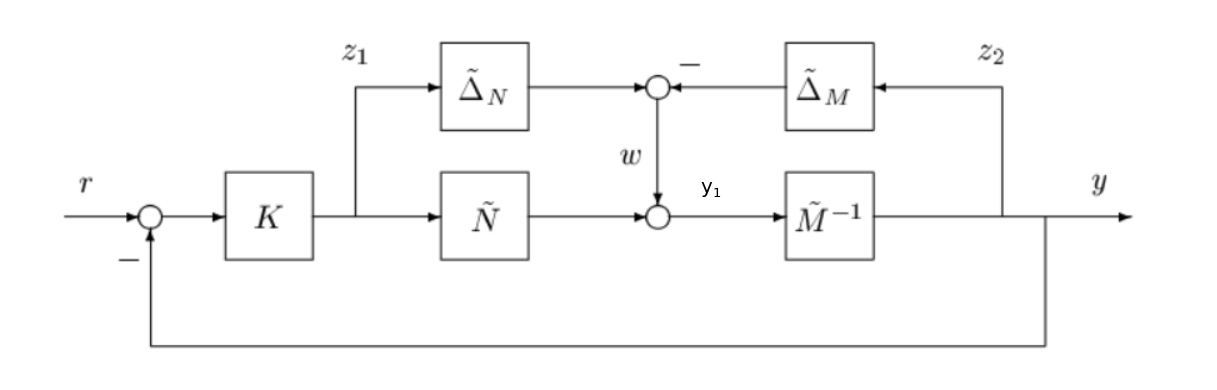
\includegraphics[scale=0.35]{co12}
%			  \includesvg[width=1.0\textwidth]{co}
%			  \def\svgscale{5.5}
%			  \tiny{
%			  \input{co2.pdf}}
			  \caption{Perturbations to Coprime Factors : Block Diagram}
			 \label{co2}
		\end{figure}	From the block diagram we have,
	
	\begin{align}
	y_{1}&=\tilde{M}y\\
	y_{1}&=\tilde{N}u + \tilde{\Delta}_{n}u - \tilde{\Delta}_{m}y\\
	\intertext{We have from these two equations, eliminating $y_{1}$} 
	y&=(\tilde{M} + \tilde{\Delta}_{m})^{-1}(\tilde{N}+\tilde{\Delta}_{n})u
	\end{align}
	Hence, the perturbed plant in this case is given by
	\begin{equation}
		\label{P1}
		P =(\tilde{M} + \tilde{\Delta}_{m})^{-1}(\tilde{N}+\tilde{\Delta}_{n})
	 \end{equation}
	 Now with this coprime factor perturbed plant, we will study the robust stabilization and the $H_{\infty}$ loop shaping controller design technique.
	\subsection{Robust Stabilization of Coprime Factors} In Eq.(\ref{P1}), we assume that $\norm{[\tilde{\Delta}_{m} \:\: \tilde{\Delta}_{n}]}_{\infty} < \epsilon$. We also assume that in Fig.(\ref{co2}) the controller $K$ internally stabilizes the nominal plant. The robust stability analysis for this system can be done by reducing the block diagram in Fig.(\ref{co2}) to LFT framework and applying the small gain theorem. For the equivalent $M-\Delta$ structure, we can obtain $M$ as follows.
	
	
	\begin{align*}
	z_{2}&=y \: ; \: z_{1} = -ky \\
	y&=\tilde{M}^{-1}(\tilde{N}u + w)\\
	\Rightarrow z_{1} &= -KPu-K\tilde{M}^{-1}w\\
	\Rightarrow z_{2} &= Gu + \tilde{M}^{-1}w\\
	y&=-PKy+\tilde{M}^{-1}w\\
	\Rightarrow y&=(I+PK)^{-1}\tilde{M}^{-1}w\\
	\Rightarrow M&=\begin{bmatrix}
	K \\ I
	\end{bmatrix}
	(I+PK)^{-1}\tilde{M}^{-1}
	\end{align*}	 
	
	Hence, on using small gain theorem, we obtain the following condition for robust stability of the system.
	\begin{equation}
	\norm{\begin{bmatrix}
	K \\ I
	\end{bmatrix}
	(I+PK)^{-1}\tilde{M}^{-1}}_{\infty} \leq \frac{1}{\epsilon}	
	\end{equation}
	
	Now, the following theorem from coprime factorization theory could be used to derive the generalized plant expression for the system shown in Fig.(\ref{co2}).
	The theorem gives the left and right coprime factorizations for a proper real-rational TFM. Let a system P have the following stabilizable and detectable minimal state space realization.
	\begin{equation}
	P =
	\begin{bmatrix}
	\begin{array}{c|c}
	A & B \\ \hline
	C & D	
	\end{array}
	\end{bmatrix}
	\label{min}
	\end{equation}
	Now, let B and L be matrices such that $A+LC$ and $A+BF$ are both stable. Then we can define:
	\begin{equation}
	\begin{bmatrix}
	M & -Y_{l} \\
	N & X_{l}
	\end{bmatrix}
	=
	\begin{bmatrix}
	\begin{array}{c|cc}
	A+BF & B & -L \\ \hline
	F & I & 0\\ 
	C+DF & D & I
	\end{array}
	\end{bmatrix}
	\end{equation}
	\begin{equation}
	\begin{bmatrix}
	X_{r} & Y_{r} \\
	-\tilde{N} & \tilde{M}
	\end{bmatrix}
	=
	\begin{bmatrix}
	\begin{array}{c|cc}
	A+LC & -(B+LD) & L \\ \hline
	F & I & 0\\ 
	C & -D & I
	\end{array}
	\end{bmatrix}
	\label{mn}
	\end{equation}
	Then $P\:=\:NM^{-1}\:=\:\tilde{M}^{-1}\tilde{N}$ are rcf and lcf respectively. The above theorem can be proved by verifying the Bezout's identity for double coprime  facotrization of plant P. Now, using Eq.(\ref{mn}), we get the following result for normalized LCF of $P$.
	\begin{equation}
	\begin{bmatrix}
	\tilde{N} & \tilde{M}
	\end{bmatrix}
	= \begin{bmatrix}
	\begin{array}{c|cc}
	A+LC & B+LD & L \\ \hline C & D & I	
	\end{array}
	\end{bmatrix}
	\label{mn2}
	\end{equation}
	Using Eq.(\ref{mn2}) and denoting the controller $\hat{K}=-K$ in Fig.(\ref{co2}), we have for $z=[z_{1}\: z_{2}]^{T}$
	\begin{align*}
	z_{1} &= u \\
	z_{2} &= \tilde{M}^{-1}w + \tilde{M}^{-1}\tilde{N}u\\
	y &= \tilde{M}^{-1}w + \tilde{M}^{-1}\tilde{N}u
	\end{align*}
	Hence, the generalized plant in the equivalent closed loop LFT structure (as shown in Fig.(\ref{lft})) is as follows (in the transfer function form).
	\begin{figure}[H]
			  \centering
			  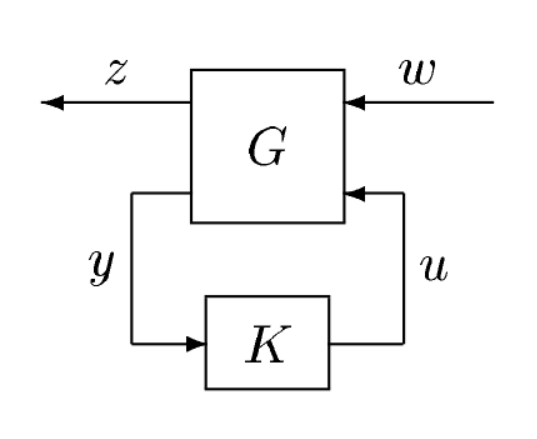
\includegraphics[scale=0.3]{lft}
%			  \includesvg[width=1.0\textwidth]{co}
%			  \def\svgscale{5.5}
%			  \tiny{
%			  \input{co2.pdf}}
			  \caption{Lower LFT Representation}
			 \label{lft}
		\end{figure}
	\begin{equation}
	G(s) = \begin{bmatrix}
	\begin{bmatrix}
	0\\\tilde{M}^{-1}
	\end{bmatrix} & \begin{bmatrix}
	I \\ P
	\end{bmatrix} \\
	\tilde{M}^{-1} & P
	\end{bmatrix}
	\label{tfnm}
	\end{equation}
	And in state space form is given by
	\begin{equation}
	G=\begin{bmatrix}
	\begin{array}{c|cc}
	A & -L & B\\ \hline
	\begin{bmatrix}
	0 \\ C
	\end{bmatrix}
	 & \begin{bmatrix}
	 0 \\I
	 \end{bmatrix}
	  & \begin{bmatrix}
	  I \\D
	  \end{bmatrix} \\
	  C & I & D
	\end{array}
	\end{bmatrix}
	\label{ssnm}
	\end{equation}
	
	Using $G(s)=C(sI-A)^{-1}B + D$ we can verify that Eq.(\ref{ssnm}) is indeed the state space representation of the TF representation given in Eq.(\ref{tfnm}).
	\[
	C= \begin{bmatrix}
	\begin{bmatrix}
	0 \\C
	\end{bmatrix} \\C
	\end{bmatrix}; 
	B=\begin{bmatrix}
	-L & B
	\end{bmatrix};
	D= \begin{bmatrix}
	\begin{bmatrix}
	0 \\I
	\end{bmatrix} & \begin{bmatrix}
	I \\ D
	\end{bmatrix} \\
	I & D
	\end{bmatrix}
	\]
	%%% WRITE STEPS%%%
	
This is an important result which would help in the design of $H_{\infty}$  loop-shaping design based controller using LMI approach. \\
 	\subsection{Design Steps}	
	$H_{\infty}$  loop shaping controller design steps were studied as presented in \cite{book}. Using pre-compensator and/or post-compensator the singular values of the nominal plant are shaped first to get a desired open loop shape. This shaped plant is represented as $G_{s}$, which is equal to $W_{2}GW_{1}$. Next, the maximum robust stability margin is calculated. It is given by
	\begin{equation}
		\epsilon_{max} = \sqrt{1-\norm{\begin{bmatrix}
		\tilde{N}_{s} & \tilde{M}_{s}\end{bmatrix}}_{H}^{2}} < 1
	\end{equation}
	where $G_{s} = \tilde{M}_{s}^{-1}\tilde{N}_{s}$ and $\tilde{M}_{s}\tilde{M}_{s}^{*} + \tilde{N}_{s}\tilde{N}_{s}^{*} = I $, i.e. $\tilde{M}_{s}$ and $\tilde{N}_{s}$ are normalized left coprime factors of the shaped plant $G_{s}$.\\
	Now, selecting $\epsilon < \epsilon_{max}$, we go ahead with the controller design based on $H_{\infty}$ optimization as follows.
	\begin{equation}
	\norm{\begin{bmatrix}
	I \\ K_{\infty}
	\end{bmatrix}
	(I+G_{s}K_{\infty})^{-1}\tilde{M}_{s}^{-1}}_{\infty} \leq \epsilon^{-1}
	\end{equation}
	The final feedback controller is given by $K=W_{1}K_{\infty}W_{2}$. The calculation of $\epsilon_{max}$, $\epsilon$ and the weights $W_{1}$ and $W_{2}$ are the choices that the designer has to make judiciously.
	%Add more to why LMI approach is helpful from the paper
	\subsection{Solvability Conditions}
		The $H_{\infty}$	 loop-shaping controller design problem using LMI approach will be described in detail in this and the next section. First, in this section, conditions for the exsitence of a suboptimal controller for the generalized plant obtained for coprime factor uncertainity description in previous section (Eq.(\ref{ssnm})) would be presented as LMIs. These existence conditions are LMIs which can be easily solved using convex optimization techniques.\\
		The key idea in deriving these existence conditions is to use the LMI based existence conditions presented in \cite{Pasca} for $H_{\infty}$ control problem by simply replacing the matrices $A$,$B_{1}$,$B_{2}$,$C_{1}$,$C_{2}$,$D_{11}$,$D_{12}$,$D_{21}$ and $D_{22}$ with those obtained for coprime factor uncertainity description (See Eq.(\ref{ssnm}))used in the design of $H_{\infty}$ loop-shaping controller. The following subsections give a detailed insight into the Theorems that would be used to derive the existence conditions. The theorems statements are as described in \cite{Pasca}.
		\subsubsection{Generalized Plant Description}
		For the LFT structure shown in Fig.(\ref{llftpk}), it has been shown in Section(\ref{lft_section}) that $T_{zw} = \mathscr{F}_{l}(P,K)$, where $\mathbb{F}_{l}(P,K) = p_{11}+p_{12}K(I-p_{22}K)^{-1}p_{21}$ for \[ P= \begin{bmatrix}
		p_{11} &p_{12}\\
		p_{21} &p_{22}
		\end{bmatrix}
		\]
		\begin{figure}[H]
			  \centering
			  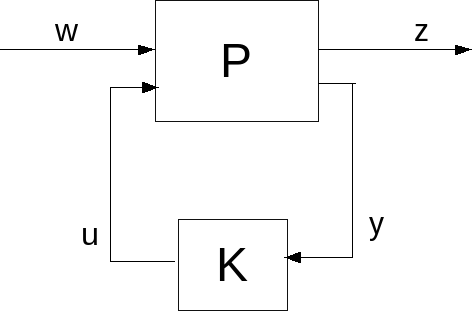
\includegraphics[scale=0.5]{llftpk}
%			  \includesvg[width=1.0\textwidth]{co}
%			  \def\svgscale{5.5}
%			  \tiny{
%			  \input{co2.pdf}}
			  \caption{Lower LFT Representation of Plant $P$ and Controller $K$}
			 \label{llftpk}
		\end{figure}	
		The above can be represented in state space form. Let $x \in \mathbb{R}^{n \times 1}$ be the state vector. For outputs $z \in \mathbb{R}^{p_{1} \times 1}$ and $y \in \mathbb{R}^{p_{2} \times 1}$ and inputs $w \in \mathbb{R}^{m_{1} \times 1}$ and $u \in \mathbb{R}^{m_{2} \times 1}$, we can write the following equations:
		\begin{align}
		\dot{x} &= Ax + B_{1}w + B_{2}u\\
		z&=C_{1}x+D_{11}w+D_{12}u\\
		y&=C_{2}x+D_{21}w+D_{22}u
		\label{ss1}
		\end{align}
		In packed matrix notation, the above can be written as follows.
		\[
		\begin{bmatrix}
		\dot{x} \\ \hline
		z\\
		y
		\end{bmatrix}
		=
		\begin{bmatrix}
	\begin{array}{c|cc}
	A & B_{1} & B_{2}\\ \hline
	C_{1}
	 & D_{11}
	  & D_{12} \\
	  C_{2} & D_{21} & D_{22}
	\end{array}
	\end{bmatrix}
	\begin{bmatrix}
	x \\ \hline
	w\\u
	\end{bmatrix}
		\]
		It is straightforward from the above discussion that $A \in \mathbb{R}^{n \times n}$, $B_{1} \in \mathbb{R}^{n \times m_{1}}$, $B_{2} \in \mathbb{R}^{n \times m_{2}}$, $C_{1} \in \mathbb{R}^{p_{1} \times n}$, $C_{2} \in \mathbb{R}^{p_{2} \times n}$, $D_{11} \in \mathbb{R}^{p_{1} \times m_{1}}$, $D_{12} \in \mathbb{R}^{p_{1} \times m_{2}}$, $D_{21} \in \mathbb{R}^{p_{2} \times m_{1}}$ and $D_{22} \in \mathbb{R}^{p_{2} \times m_{2}}$. Next, the controller can be written as follows:
		\[
		K=\begin{bmatrix}
		\begin{array}{c|c}
		A_{k} & B_{k} \\ \hline
		C_{k} & D_{k}
		\end{array}
		\end{bmatrix}
		\]
		where $A_{k} \in \mathbb{R}^{k \times k}$, $B_{k} \in \mathbb{R}^{k \times p_{2}}$, $C_{k} \in \mathbb{R}^{m_{2} \times k}$ and $D_{k} \in \mathbb{R}^{m_{2} \times p_{2}}$ are the state matrices for the controller $K$, where $u=K(s)y$. We can also write,
		\begin{align}
		\dot{x}_{k} &= A_{k}x_{k} + B_{k}y\\
		u&=C_{k}x_{k}+D_{k}y
		\label{ss2}
		\end{align}
		\\
		We begin by writing the closed loop structure shown in Fig. (\ref{llft}) in state space form. This can be done by absorbing the controller $K$ into the state space representation to obtain the following:
		\begin{equation}
		\begin{bmatrix}
		\dot{x} \\
		\dot{x}_{k} \\ \hline
		z
		\end{bmatrix}
		=
		\begin{bmatrix}
	\begin{array}{c|c}
	A_{cl} & B_{cl}\\ \hline
	C_{cl}
	 & D_{cl}
	\end{array}
	\end{bmatrix}
	\begin{bmatrix}
	x \\ x_{k} \\ \hline
	w
	\end{bmatrix}
	\label{cl}
		\end{equation}
		where the closed loop transfer function from $w$ to $z$ is given by \\ $\mathscr{F}(P,K)(s) = C_{cl}(sI-A_{cl})^{-1}B_{cl} + D_{cl}$. We will next show the derivation of these closed loop matrices.
		\\
		\begin{align*}
		u&=Ky \\
		\intertext{From Eq.(\ref{ss1}) and (\ref{ss2}), we have}
		y &= C_{2}x + D_{21}w+D_{22}C_{k}x_{k} + D_{22}D_{k}y\\
		\Rightarrow y &= (I-D_{22}D_{k})^{-1}C_{2}x + (I-D_{22}D_{k})^{-1}D_{21}w  + (I-D_{22}D_{k})^{-1}D_{22}C_{k}x_{k} \\
		z&=C_{1}x+D_{11}w+D_{12}C_{k}x_{k}+D_{12}D_{k}y\\
		\Rightarrow z&=(C_{1} + D_{12}D_{k}(I-D_{22}D_{k})^{-1}C_{2})x+ (D_{12}C_{k}+ D_{12}D_{k}(I-D_{22}D_{k})^{-1}D_{22}C_{k})x_{k} + \\& (D_{11}w+D_{12}D_{k}(I-D_{22}D_{k})^{-1}D_{21})w\\
		\dot{x}&=Ax+B_{1}w+B_{2}C_{k}x_{k} + B_{2}D_{k}(I-D_{22}D_{k})^{-1}C_{2}x+ B_{2}D_{k}(I-D_{22}D_{k})^{-1}D_{21}w + \\& B_{2}D_{k}(I-D_{22}D_{k})^{-1}D_{22}C_{k}x_{k}\\
		\Rightarrow \dot{x} &= (A+B_{2}D_{k}(I-D_{22}D_{k})^{-1}C_{2})x+(B_{2}C_{k}+ B_{2}D_{k}(I-D_{22}D_{k})^{-1}D_{22}C_{k})x_{k} + \\& (B_{1} + B_{2}D_{k}(I-D_{22}D_{k})^{-1}D_{21})w\\
		\dot{x}_{k}&=A_{k}x_{k} + B_{k}(I-D_{22}D_{k})^{-1}C_{2}x + B_{k}(I-D_{22}D_{k})^{-1}D_{12}C_{k}x_{k}+ \\&B_{k}(I-D_{22}D_{k})^{-1}D_{21}w
		\end{align*}
		Using the above equations, we can find out $A_{cl}$, $B_{cl}$, $C_{cl}$ and $D_{cl}$ to satisfy Eq.(\ref{cl}). 
		\[
		A_{cl} = \begin{bmatrix}
		A + B_{2}D_{k}(I-D_{22}D_{k})^{-1}C_{2} & B_{2}C_{k} + B_{2}D_{k}(I-D_{22}D_{k})^{-1}D_{22}C_{k} \\
		B_{k}(I-D_{22}D_{k})^{-1}C_{2} & A_{k} + B_{k}(I-D_{22}D_{k})^{-1}D_{22}C_{k}
		\end{bmatrix}
		\]
		\[
		B_{cl} = \begin{bmatrix}
		B_{1}+B_{2}D_{k}(I-D_{22}D_{k})^{-1}D_{21} \\
		B_{k}(I-D_{22}D_{k})^{-1}D_{21}
		\end{bmatrix}
		\]
		\[
		C_{cl} = \begin{bmatrix} 
		C_{1} + D_{12}D_{k}(I-D_{22}D_{k})^{-1}C_{2} & D_{12}C_{k} + D_{12}D_{k}(I-D_{22}D_{k})^{-1}D_{22}C_{k}
		\end{bmatrix}
		\]
		\[
		D_{cl}=D_{11}+D_{12}D_{k}(I-D_{22}D_{k})^{-1}D_{21}
		\]
		
		Also, as it is clear that if $D_{22}$ is chosen as a null matrix the above equations are simplified to a great extent. So, taking $D_{22} = 0$, we get:

		\[
		A_{cl} = \begin{bmatrix}
		A + B_{2}D_{k}C_{2} & B_{2}C_{k} \\
		B_{k}C_{2} & A_{k}
		\end{bmatrix},
		B_{cl} = \begin{bmatrix}
		B_{1}+B_{2}D_{k}D_{21} \\
		B_{k}D_{21}
		\end{bmatrix}
		\]
		\[
		C_{cl} = \begin{bmatrix} 
		C_{1} + D_{12}D_{k}C_{2} & D_{12}C_{k}
		\end{bmatrix},
		D_{cl}=D_{11}+D_{12}D_{k}D_{21}
		\]
		Hence, $D_{22}=0$ is one of the assumptions in the LMI approach to $H_{\infty}$ controller design. Also, we can simplify the above matrices by using the following notation:
		\begin{align}
		\label{not}
		&A_{0} (\in \mathbb{R}^{(n+k) \times (n+k)})= \begin{bmatrix}
		A & 0 \\ 0 & 0_{k \times k}
		\end{bmatrix};
		B_{0} (\in \mathbb{R}^{(n+k) \times (m_{1})})= \begin{bmatrix}
		B_{1} \\ 0_{k \times m_{1}}
		\end{bmatrix}\\
		&C_{0} (\in \mathbb{R}^{(p_{1}) \times (n+k)})= \begin{bmatrix}
		C_{1} & 0_{p_{1} \times k}
		\end{bmatrix};
		\mathscr{B} (\in \mathbb{R}^{(n+k) \times (m_{2}+k)})=\begin{bmatrix}
		0_{n \times k} & B_{2} \\ I_{k} & 0_{k \times m_{2}}
		\end{bmatrix}
		\\
		&\mathscr{C}(\in \mathbb{R}^{(p_{2}+k) \times (n+k)}) = \begin{bmatrix}
		0_{k \times n} & I_{k} \\
		C_{2} & 0_{p_{2} \times k}
		\end{bmatrix};
		\mathscr{D}_{12}(\in \mathbb{R}^{(p_{1}) \times (m_{2}+k)}) = \begin{bmatrix}
		0_{p_{1} \times {k}} & D_{12}
		\end{bmatrix}\\
		&\mathscr{D}_{21}(\in \mathbb{R}^{(p_{2}+k) \times (m_{1})})= \begin{bmatrix}
		0_{k \times m_{1}} \\ D_{21}
		\end{bmatrix}
		\end{align}
		This notation is helpful because it only depends on plant data and as we will see in the following expression the closed loop matrices will depend affinely on controller data if the above notation is used.
		\[
		A_{cl} (\in \mathbb{R}^{(n+k) \times (n+k)})=A_{0}+\mathscr{B}\theta\mathscr{C};
		B_{cl}(\in \mathbb{R}^{(n+k) \times m_{1}})=B_{0}+\mathscr{B}\theta\mathscr{D}_{21}
		\]
		\[
		C_{cl}(\in \mathbb{R}^{p_{1} \times (n+k)})=C_{0}+\mathscr{D}_{12}\theta\mathscr{C};
		D_{cl}(\in \mathbb{R}^{p_{1} \times m_{1}})=D_{11}+\mathscr{D}_{12}\theta\mathscr{D}_{21};
		\]
		where 
		\[
		\theta (\in \mathbb{R}^{(m_{2}+k) \times (p_{2}+k)})= \begin{bmatrix}
		A_{k} & B_{k} \\ C_{k} & D_{k}
		\end{bmatrix}
		\]
		The above can be verified by simple substitution. \\
		Other than the assumption that $D_{22}=0$, we also assume that the plant is stabilizable and detectable. Hence, using LMI approach to design $H_{\infty}$ controller only these two assumptions are needed. This is one of the advantages of the LMI approach compared to the DGKF method as mentioned in previous sections. Now, we present the solvability conditions for the existence of a suboptimal controller for the generalized plant described above.
		\subsubsection{Controller Existence Conditions}
		\paragraph{Theorem 1}
		Consider the proper plant $P(s)$ and assume that the two assumptions mentioned above hold true. Define
		\begin{align}
		\label{P}
		\mathscr{P}:=
		\begin{bmatrix}
		\mathscr{B}^{T} & 0_{(k+m_{2})\times m_{1}} & \mathscr{D}_{12}^{T}
		\end{bmatrix} \\
		\label{D}
		\mathscr{D}:=
		\begin{bmatrix}
		\mathscr{C} & \mathscr{D}_{21} & 0_{(k+p_{2})\times p_{1}}
		\end{bmatrix}
		\end{align}
		and let $W_{\mathscr{P}}$ and $W_{\mathscr{D}}$ be the basis of null spaces of $\mathscr{P}$ and $\mathscr{D}$, respectively. Then the set of $\gamma-$suboptimal controllers of order $k$ is nonempty iff there exists some $(n+k) \times (n+k)$ positive definite matrix $X_{cl}$ such that:
		\begin{align}
		\label{th1eq1}
		W_{\mathscr{P}}^{T}\Phi_{X_{cl}}W_{\mathscr{P}} < 0 \\ 
		\label{th1eq2}
		W_{\mathscr{D}}^{T}\Psi_{X_{cl}}W_{\mathscr{D}} < 0
		\end{align}
		where
		\begin{equation}
		\Phi_{X_{cl}} :=
		\begin{bmatrix}
			A_{0}X_{cl}^{-1}+X_{cl}^{-1}A_{0}^{T} & B_{0} & X_{cl}^{-1}C_{0}^{T} \\
			B_{0}^{T} & -\gamma I & D_{11}^{T} \\
			C_{0}X_{cl}^{-1} & D_{11} & -\gamma I
		\end{bmatrix}
		\label{phixcl}
		\end{equation}
		\begin{equation}
		\Psi_{X_{cl}} :=
		\begin{bmatrix}
			A_{0}^{T}X_{cl}+X_{cl}A_{0} & X_{cl}B_{0} & C_{0}^{T} \\
			B_{0}^{T}X_{cl} & -\gamma I & D_{11}^{T} \\
			C_{0} & D_{11} & -\gamma I
		\end{bmatrix}
		\label{sixcl}
		\end{equation}
		Proof: \\
		From the Bounded Real Lemma described in Section(\ref{brl}), for some matrix $X_{cl} = X_{cl}^{T} > 0 \in \mathbb{R}^{(n+k) \times (n+k)}$, we can write that $\norm{G_{cl}}_{\infty} < \gamma$ is equivalent to
		\begin{equation}
		\begin{bmatrix}
		A_{cl}^{T}X_{cl}+X_{cl}A_{cl} & X_{cl}B_{cl} & C_{cl}^{T} \\
			B_{cl}^{T}X_{cl} & -\gamma I & D_{cl}^{T} \\
			C_{cl} & D_{cl} & -\gamma I
		\end{bmatrix}
		< 0
		\label{xcl}
		\end{equation}
		where $G_{cl}$ in packed matrix notation can be written as,
		\[
		G_{cl}= \begin{bmatrix}
		\begin{array}{c|c}
	A_{cl} & B_{cl}\\ \hline
	C_{cl}
	 & D_{cl}
	\end{array}
	\end{bmatrix}.
	\]
	Now, using Eq.(\ref{sixcl}) and notation given in (\ref{not}), we can write Eq.(\ref{xcl}) as follows:
	\[
	\begin{bmatrix}
	A_{0}^{T}X_{cl} + \mathscr{C}^{T}\theta^{T}\mathscr{B}^{T}X_{cl} + X_{cl}A_{0}+X_{cl}\mathscr{B}\theta\mathscr{C} & X_{cl}B_{0} + X_{cl}\mathscr{B}\theta\mathscr{D}_{21} & C_{0}^{T} + \mathscr{C}^{T}\theta^{T}\mathscr{D}_{12}^{T} \\
	B_{0}^{T}X_{cl} + \mathscr{D}_{21}^{T}\theta^{T}\mathscr{B}^{T}X_{cl} & -\gamma I & D_{11}^{T} + \mathscr{D}_{21}^{T}\theta^{T}\mathscr{D}_{12}^{T} \\
	C_{0} + \mathscr{D}_{12}\theta\mathscr{C} & D_{11} + \mathscr{D}_{12}\theta\mathscr{D}_{21} & -\gamma I 
	\end{bmatrix}
	<0
	\]
	Now observing that,
	\[
	\mathscr{D}^{T}\theta^{T}\mathscr{P}_{X_{cl}} = 
	\begin{bmatrix}
	\mathscr{C}^{T}\theta^{T} \\ \mathscr{D}_{21}\theta^{T} \\ 0
	\end{bmatrix}
	\begin{bmatrix}
	\mathscr{B}^{T}X_{cl} & 0 & \mathscr{D}_{12}^{T}
	\end{bmatrix}
	=
	\begin{bmatrix}
	\mathscr{C}^{T}\theta^{T}\mathscr{B}^{T}X_{cl} & 0 & \mathscr{C}^{T}\theta^{T}\mathscr{D}_{12}^{T} \\
	\mathscr{D}_{21}\theta^{T}\mathscr{B}^{T}X_{cl} & 0 & \mathscr{D}_{21}\theta^{T}\mathscr{D}_{12}^{T}\\
	0 & 0 & 0
	\end{bmatrix}
	\]
	We have,
	\begin{equation}
	\Psi_{X_{cl}} + \mathscr{D}^{T}\theta^{T}\mathscr{P}_{X_{cl}} + \mathscr{P}_{X_{cl}}^{T}\theta\mathscr{D} < 0 
	\label{A}
	\end{equation}
	This equation is solvable if and only if,
	\begin{align}
	\label{tophi}
	W_{\mathscr{P}_{X_{cl}}}^{T}\Psi_{X_{cl}}W_{\mathscr{P}_{X_{cl}}} < 0 
	W_{\mathscr{D}}^{T}\Psi_{X_{cl}}W_{\mathscr{D}} < 0 
	\end{align}
	where  $W_{\mathscr{P}_{X_{cl}}}$ and $W_{\mathscr{D}}$ are the basis of the null spaces of $\mathscr{P}_{X_{cl}}$ and $\mathscr{D}$ respectively. For the proof of this lemma, the reader is referred to Section 3 of \cite{Pasca}.
	Now, we will reduce the Eq. (\ref{tophi}) as follows to prove the statement of the theorem.
	\begin{align*}
		I&=\begin{bmatrix}
		X_{cl} & 0 & 0 \\
		0 & I & 0 \\
		0 & 0 & I
		\end{bmatrix}
		\begin{bmatrix}
		X_{cl}^{-1} & 0 & 0 \\
		0 & I & 0 \\
		0 & 0 & I
		\end{bmatrix} \\
		\intertext{So, we can write,}
		\mathscr{P} &= \mathscr{P}_{X_{cl}}\begin{bmatrix}
		X_{cl}^{-1} & 0 & 0 \\
		0 & I & 0 \\
		0 & 0 & I
		\end{bmatrix}	\\
	\intertext{Using the above and finding basis of the null spaces, we have,}
	W_{\mathscr{P}_{X_{cl}}} &= \begin{bmatrix}
	X_{cl}^{-1} & 0 & 0 \\
		0 & I & 0 \\
		0 & 0 & I
	\end{bmatrix} W_{\mathscr{P}}\\
	\intertext{where $W_{\mathscr{P}_{X_{cl}}}$ and $ W_{\mathscr{P}}$ are the basis of the null space of $\mathscr{P}_{X_{cl}}$ and $\mathscr{P}$ respectively. Now, rewriting Eq.(\ref{tophi}), we get}
	W_{\mathscr{P}}^{T}&\left(\begin{bmatrix}
	X_{cl}^{-1} & 0 & 0 \\
		0 & I & 0 \\
		0 & 0 & I
	\end{bmatrix}
	\Psi_{X_{cl}} \begin{bmatrix}
	X_{cl}^{-1} & 0 & 0 \\
		0 & I & 0 \\
		0 & 0 & I
	\end{bmatrix}\right)
	W_{\mathscr{P}} < 0\\
	\intertext{Simplifying, we finally get,}
		W_{\mathscr{P}}^{T}&\Phi_{X_{cl}}W_{\mathscr{P}} < 0
	\end{align*}		
	Hence, the theorem is proved. The next theorem eradicates the need to compute $X_{cl}^{-1}$ and also shows the role of plant parameters in the solvability conditions.
	\paragraph{Theorem 2}
	Consider a continuous time plant $P(s)$ of order $n$ and minimal realization given in Eq.(\ref{min}). Let $\mathscr{N}_{R}$ and $\mathscr{N}_{S}$ be bases of null space of $(B_{2}^{T}, D_{12}^{T})$ and $(C_{2},D_{21})$ respectively. The suboptimal $H_{\infty}$ problem of parameter $\gamma$ is solvable if and only if the following three conditions (formulated in LMI) are satisfied.
	\begin{align}
	\label{th2eq1}
	\begin{bmatrix}
	\mathscr{N}_{R} & 0 \\
	0 & I
	\end{bmatrix}^{T}
	\begin{bmatrix}
	AR+RA^{T} & RC_{1}^{T} & B_{1} \\
	C_{1}R & -\gamma I & D_{11} \\
	B_{1}^{T} & D_{11}^{T} & -\gamma I
	\end{bmatrix}
	\begin{bmatrix}
	\mathscr{N}_{R} & 0 \\
	0 & I
	\end{bmatrix} &<0 \\
	\label{th2eq2}
	\begin{bmatrix}
	\mathscr{N}_{S} & 0 \\
	0 & I
	\end{bmatrix}^{T}
	\begin{bmatrix}
	A^{T}S+SA & SB_{1} & C_{1}^{T} \\
	B_{1}^{T}S & -\gamma I & D_{11}^{T} \\
	C_{1} & D_{11} & -\gamma I
	\end{bmatrix}
	\begin{bmatrix}
	\mathscr{N}_{S} & 0 \\ 
	0 & I
	\end{bmatrix} &<0 \\
	\label{th2eq3}
	\begin{bmatrix}
	R & I\\I & S
	\end{bmatrix} &\geq 0
	\end{align}
	\textbf{Proof:} Our main aim with this Theorem is to express the existence conditions derived in Theorem 1 in terms of plant parameters. We express $X_{cl}$ and $X_{cl}^{-1}$ as follows
	\begin{equation}
	X_{cl} := \begin{bmatrix}
	S & N \\
	N^{T} & *
	\end{bmatrix}; \: \:
	X_{cl}^{-1} := \begin{bmatrix}
	R & M \\
	M^{T} & *
	\end{bmatrix}
	\label{Xcl_partition}
	\end{equation}
	where $R,S \in \mathbb{R}^{n \times n}$ and $M, N \in \mathbb{R}^{n \times k}$. 
Consider Eq.(\ref{th1eq1}) and substitute $X_{cl}$ from Eq.(\ref{Xcl_partition}). We have,
	\begin{equation}
	\Phi_{X_{cl}} = \begin{bmatrix}
	AR+RA^{T} & AM & B_{1} & RC_{1}^{T} \\
	M^{T}A^{T} & 0 & 0 & M^{T}C_{1}^{T} \\
	B_{1}^{T} & 0 & -\gamma I & D_{11}^{T} \\
	C_{1}R & C_{1}M & D_{11} & -\gamma I
	\end{bmatrix}
	\label{phixcl_part}
	\end{equation}
	From Eq.(\ref{P}), we can find out the basis of null space of $\mathscr{P}$ in the following form
	\[
	W_{\mathscr{P}} = \begin{bmatrix}
	W_{1} & 0\\
	0 & 0 \\
	0 & I_{m_{1}} \\
	W_{2} & 0
	\end{bmatrix}
	\]
	where 
	\[
	\mathscr{N}_{R} := \begin{bmatrix}
	W_{1} \\ W_{2}
	\end{bmatrix}
	\] is any basis of null space of $\begin{bmatrix}
	B_{2}^{T} & D_{12}^{T}
	\end{bmatrix}$. \\
	Above can be found out be finding indiviudal elements of $W_{\mathscr{P}}$ that satisfy the following which make $W_{\mathscr{P}}$  the basis of null space of $\mathscr{P}$.
	\begin{equation}
	\mathscr{P}W_{\mathscr{P}} = 0
	\end{equation}
	Now, the Eq.(\ref{th1eq1}) can be reduced using the above and Eq.(\ref{phixcl_part}) to read as given below:
	\begin{align}
	\begin{bmatrix}
	W_{1} & 0 \\ 0 & I_{m_{1}} \\ W_{2} & 0 
	\end{bmatrix}^{T}
	\begin{bmatrix}
	AR + RA^{T} & B_{1} & RC_{1}^{T} \\
	B_{1}^{T} & -\gamma I & D_{11}^{T} \\
	C_{1}R & D_{11} & -\gamma I
	\end{bmatrix}
	\begin{bmatrix}
	W_{1} & 0 \\ 0 & I_{m_{1}} \\ W_{2} & 0 
	\end{bmatrix} &< 0 \\
	\intertext{Substituting for $W_{1}$ and $W_{2}$ from above, we can write}
	\begin{bmatrix}
	\mathscr{N}_{R} & 0 \\
	0 & I
	\end{bmatrix}^{T}
	\begin{bmatrix}
	AR+RA^{T} & RC_{1}^{T} & B_{1} \\
	C_{1}R & -\gamma I & D_{11} \\
	B_{1}^{T} & D_{11}^{T} & -\gamma I
	\end{bmatrix}
	\begin{bmatrix}
	\mathscr{N}_{R} & 0 \\ 
	0 & I
	\end{bmatrix} &<0 
	\end{align}
	which proves the first statement of the Theorem given in Eq.(\ref{th2eq1}). \\Using a similar approach we will next prove the second statement of the Theorem in Eq.(\ref{th2eq2}). Consider Eq.(\ref{th1eq2}), i.e. $W_{\mathscr{D}}\Psi_{X_{cl}}W_{\mathscr{D}} < 0 $. We will reduce this equation of Theorem 1 in the terms of plant parameters. From Eq.(\ref{Xcl_partition}), we can write $\Psi_{X_{cl}}$ as follows:
	\begin{align}
	\Psi_{X_{cl}} &= \begin{bmatrix}
	A^{T}S + SA & A^{T}N & SB_{1} & C_{1}^{T} \\
	N^{T}A & 0 & N^{T}B_{1} & 0 \\
	B_{1}^{T}S & B_{1}^{T}N & -\gamma I & D_{11}^{T} \\
	C_{1} & 0 & D_{11} & -\gamma I
	\end{bmatrix} \\
	\intertext{From Eq.(\ref{D}), we have}
	\mathscr{D} &= \begin{bmatrix}
	0_{k \times n} & I_{k \times k} & 0_{k \times m_{1}} & 0_{k \times p_{1}} \\
	C_{2_{p_{2} \times n}} & 0_{p_{2} \times k} & D_{21_{p_{2} \times m_{1}}} & 0_{p_{2} \times p_{1}}
	\end{bmatrix}\\
	\intertext{Using the above, and using the proper dimensions as mentioned above to solve $\mathscr{D}W_{\mathscr{D}} = 0$ to get $\mathscr{W}_{\mathscr{D}}$, the basis of null space of $\mathscr{D}$. We get}
	W_{\mathscr{D}} &= \begin{bmatrix}
	W_{3} & 0 \\
	0 & 0 \\
	W_{4} & 0 \\
	0 & I
	\end{bmatrix} \\
	\intertext{where}
	\mathscr{N}_{S} &= \begin{bmatrix}
	W_{3} \\ W_{4}
	\end{bmatrix}\\
	\intertext{is the basis of null space of $\begin{bmatrix}
	C_{2} & D_{21}
	\end{bmatrix}$. Substituting, we get,}
	&\begin{bmatrix}
	\mathscr{N}_{S} & 0 \\
	0 & I
	\end{bmatrix}^{T}
	\begin{bmatrix}
	A^{T}S+SA & SB_{1} & C_{1}^{T} \\
	B_{1}^{T}S & -\gamma I & D_{11}^{T} \\
	C_{1} & D_{11} & -\gamma I
	\end{bmatrix}
	\begin{bmatrix}
	\mathscr{N}_{S} & 0 \\ 
	0 & I
	\end{bmatrix} <0
	\end{align}	 
	The third statement in Eq.(\ref{th2eq3}) is clearly seen as $X_{cl}>0$ and from Eq.(\ref{Xcl_partition}), we get $R$ and $S$ satisfying Eq.(\ref{th2eq3}). Hence, we have proved the Theorem to obtain the existence conditions for a $\gamma$-suboptimal $H_{\infty}$ controller formulated in LMI. Next, we will use these conditions to derive the conditions for existence for $H_{\infty}$ loop-shaping design.
	 	\subsubsection{Conditions for $H_{\infty}$ loop-shaping design}
	 	For the generalized plant expression obtained for coprime factor uncertainity description to design an $H_{\infty}$ loop-shaping controller, we can obtain the solvability conditions for existence of a $\gamma$-suboptimal controller as follows.
	 	From the generalized plant expression in Eq.(\ref{ssnm}) we have.
	 	\begin{align}
	 	B_{2}&=B_{n \times p} ; D_{12} = \begin{bmatrix}
	 	I_{p} \\ 0_{m \times p}
	 	\end{bmatrix} \\
	 	\intertext{To find $\mathscr{N}_{R}$, i.e. the basis of null space of $\begin{bmatrix}
	 	B_{2}^{T} & D_{12}^{T}
	 	\end{bmatrix}$ we have the rank of null space $= (n+m)$ and $\mathscr{N}_{R} \in \mathbb{R}^{(n+p+m) \times (n+m)}$. We get}
	 	\mathscr{N}_{R} &= \begin{bmatrix}
	 	I_{n} & 0_{n \times m} \\
	 	-B^{T}_{p \times n} & 0_{p \times m}\\
	 	0_{m \times n} & I_{m}
	 	\end{bmatrix}\\
	 	\intertext{Similarly, we see that for $\mathscr{N}_{S}$, the basis of null space of $\begin{bmatrix}
	 	C_{2} & D_{21}
	 	\end{bmatrix}$, we have for $H_{\infty}$ loop-shaping design from Eq.(\ref{ssnm})}
	 	C_{2}&=C_{m \times n} \: ; \: D_{21}=I_{m} \\
	 	\intertext{The rank of $\mathscr{N}_{S} \in \mathbb{R}^{(m+n) \times n}$ hence will be equal to $n$. We can then write}
	 	\mathscr{N}_{S} &= \begin{bmatrix}
	 	I_{n} \\ -C_{m \times n}
	 	\end{bmatrix}
	 	\end{align}
	 	 	\subsubsection{LMI Formulation}
	 	From $\mathscr{N}_{R}$ and $\mathscr{N}_{S}$ obtained above, we can reduce the solvability conditions for the existence of a suboptimal $H_{\infty}$ loop-shaping controller as three LMIs given below. These three LMIs can be solved to find out the value of $\gamma$, $R$ and $S$ which can then be used to design the controller as shown in the following section. The three LMIs which need to be solved for $R$, $S$ and $\gamma$ are:
	 	\begin{align}
	 	\begin{bmatrix}
	 	AR + RA^{T} - \gamma BB^{T} & RC^{T} & -L\\
	 	CR & -\gamma I & I \\
	 	-L^{T} & I & -\gamma I 
	 	\end{bmatrix} &< 0 \\
	 	A^{T}S + SA + C^{T}L^{T}S + SLC - \gamma C^{T}C &< 0 \\
	 	\begin{bmatrix}
	 	R & I \\
	 	I & S
	 	\end{bmatrix} &\geq 0
	 	\end{align}
	 	Other than the three convex conditions mentioned above, if we want to ensure that the obtained controller is of order $k$ where $k<n$, then another conditions should be satisfied.
	 	\begin{center} Rank$(I-RS) \leq k$ \end{center}
	 	Some examples simulating a few physical systems on MATLAB to solve the above equation are presented in the next section.
	 	\subsection{Examples and Simulations}
	 	The controller solvability conditions LMIs for a few numerical examples and physical systems have been solved and presented in this section. 
	 		\subsubsection{A BLDC Hub Motor Driving a Three Wheeled Mobile Robot}
	 		Consider a tricycle model of a mobile robot driven by a BLDC hub motor. As an over-simplistic model of the robot, we consider modeling the velocity control of the BLDC motor only.\\
	 	Using system identification technique in MATLAB with the data of the input voltage to the motor and the output velocity measurements, the following estimated TF was obtained. We will show that an $H_{\infty}$ loop-shaping controller design can be done by showing the existence of the $\gamma$-suboptimal controller by solving the LMIs developed in previous section.
	 	The plant model is given by,
	 	\begin{align}
	 	G(s)&= \frac{0.001011s^{2} + 0.0006967{s} + 1.801 \times 10^{-6}}{s^{3} + 1.16 s^{2} + 0.3351s + 0.007859}\\
	 	\intertext{To obtain the shaped plant, we choose a first order weight $W_{1}$ as follows and $W_{2}=1$ is chosen}
	 	W_{1}(s) &= \frac{10s + 3}{s(s + 8)}\\
	 	\intertext{Using the above, we find the following  minimal state space representation of the shaped plant. Using this, we solve the LMIs formulated in the previous section}
	 	A& =\begin{bmatrix}
  -9.1600  & -2.4038 &  -0.6722  & -0.0157        & 0\\
    4.0000    &     0     &    0       &  0        & 0 \\
         0   & 1.0000    &     0       &  0        & 0 \\
        0    &     0   & 1.0000       &  0        & 0 \\
       0     &    0        & 0   & 1.0000        & 0 \\
\end{bmatrix} ; \:
B =
\begin{bmatrix}
    0.0625\\
         0\\
         0\\
         0\\
         0\\
\end{bmatrix}\\
C &= \begin{bmatrix}
         0    & 0.0404 &    0.0400 &   0.0084  &  0.0000
\end{bmatrix}; \:
D = 0
	 	\end{align}
	 The valus of $\gamma$ obtained on solving the LMIs is $1.3937$. We take another similar example next. 
	 \subsubsection{A Wheeled Mobile Robot System}
	 A second order SISO model (simplified) of a wheeled mobile robot has been derived in \cite{robot}. We use the TF model given to check if a $\gamma$-suboptimal $H_{\infty}$ loop-shaping controller exists for the system or not. 
	 \begin{align}
	 G(s)&=\frac{0.3961}{0.2256s^{2} + 0.3645s + 1.469} \\
	 \intertext{With the same weights as in previous example, we get the minimal state space realization of the shaped plant as follows}
	 A &=
\begin{bmatrix}
   -1.6157  & -3.2558  &  2.5000   & 0.7500 \\
    2.0000     &    0   &      0    &     0\\
         0    &     0  & -8.0000   &      0\\
         0   &      0  &  1.0000  &       0
\end{bmatrix}; \:
B =
\begin{bmatrix}
     0\\
     0\\
     4\\
     0
\end{bmatrix}\\
C &=
\begin{bmatrix}
         0  &  0.8779       &  0       &  0
\end{bmatrix}; \:
D =     0
     \end{align}
     Solving the LMIs we get the value of $\gamma=1.2761$. 
     \subsubsection{F-16 Fighter Aircraft Model} 
     Finally, we show a MIMO system example. The longitudinal model of a F-16 fighter aircraft is shown below. The state space representation as shown below has been taken from \cite{aircraft} Pages 370-371. For details on definition of states, the equilibrium point about which linearization is done and other details the reader is referred to \cite{aircraft}.
     \begin{align}
     A &= \begin{bmatrix}
-0.3220 & 0.0640 & 0.0364 & -0.9917 & 0.0003 & 0.0008 & 0\\
0 &0 &1 &-0.0037 &0 &0 &0\\
-30.6492 &0 &-3.6784 &0.6646 &-0.7333 &0.1315 &0\\
8.5396 &0 &-0.0254 &-0.4764 &-0.0319 &-0.0620 &0\\
0 &0 &0 &0 &-20.2 &0 &0\\
0 &0 &0 &0 &0 &-20.2 &0\\
0 &0 &0 &57.2958 &0 &0 &-1 \end{bmatrix}\\
B &= \begin{bmatrix}
0& 0 \\
0& 0\\
0& 0\\
0& 0\\
20.2 &0\\
0 &20.2\\
0 &0 \end{bmatrix}\\
C &= \begin{bmatrix}
0 &0 &0 &57.2958 &0 &0 &-1\\
0 &0 &57.2958 &0 &0 &0 &0\\
57.2958 &0 &0 &0 &0 &0 &0\\
0& 57.2958 &0 &0 &0 &0 &0 \end{bmatrix};\: D=[0]_{4 \times 2}
     \end{align}
Solving the LMIs we obtain $\gamma=3.1587$. With this we move on to controller design at the end of which we will show $H_{\infty}$ controller design for these physical systems.      
	 \subsection{Controller Design}
	 Using the Bounded Real Lemma developed in Section \ref{brl} and solving the corresponding LMI, we can find out the controller by using the values of $R$ and $S$ obtained by solving the controller existence conditions. The steps to reconstruct the controller are given below.
	 \begin{enumerate}
	 \item Compute two full column rank matrices $M$ and $N$ such that
	 \begin{equation}
	 MN^{T} = I - RS
	 \end{equation}
	 \item From the matrices $M$ and $N$ calculated in the first step, $X_{cl}$ can be found out as follows. Recall that, as defined previously, $X_{cl}$ is a positive definite matrix $\in \mathbb{R}^{(n+k) \times (n+k)}$ which satisfies Eq. (\ref{Xcl_partition}). Solving the following equation, $X_{cl}$ can be computed.
	 \begin{equation}
	 \begin{bmatrix}
	 S & I \\ N^{T} & 0
	 \end{bmatrix}
	 =
	 X_{cl}\begin{bmatrix}
	 I & R \\
	 0 & M^{T}
	 \end{bmatrix}
	 \label{Xcl}
	 \end{equation}
	 Note that Eq.(\ref{Xcl}) is always solvable when $S>0$ and $M$ has full column rank. 
	\item As seen in Theorem 1, from Eq.(\ref{xcl}) we can solve the following Bounded Real Lemma inequality:
	\begin{equation}
		\begin{bmatrix}
			A_{cl}^{T}X_{cl}+X_{cl}A_{cl} & X_{cl}B_{cl} & C_{cl}^{T} \\
			B_{cl}^{T}X_{cl} & -\gamma I & D_{cl}^{T} \\
			C_{cl} & D_{cl} & -\gamma I
		\end{bmatrix}
		=\Psi_{X_{cl}} + \mathscr{D}^{T}\theta^{T}\mathscr{P}_{X_{cl}}+\mathscr{P}_{X_{cl}}^{T}\theta\mathscr{D} <0
		\end{equation}
	\item The above LMI can be solved for $\theta$ to obtain the controller parameters. 
	\begin{equation}
	\theta = \begin{bmatrix}
	A_{k} & B_{k} \\
	C_{k} & B_{k}
	\end{bmatrix}.
	\end{equation}
	 \end{enumerate}
	 
	\section{Conclusion and Future Work}

In this project we covered the basics of robust control theory and studied the theory towards general $H_{\infty}$ control framework. Using which, $H_{\infty}$ loop-shaping design procedure was studied.\\ The project initially dealt with robustness analysis of uncertain systems. The linear fractional transformation theory which is widely used to represent all systems with uncertainities was studied. Using the LFT framework, many systems were modeled. A common physical system, the spring mass damper, with parametric uncertainities was expressed as an LFT and robustness analysis for the same was done. Subsequently, based on the performance and robust stability specifications, general $H_{\infty}$ problem was formulated.  \\After the analysis, controller design was considered using LMI approach which is computationally more efficient than conventional $H_{\infty}$ controller design methods. Finally, an $H_{\infty}$ loop-shaping controller design procedure using LMI approach was demonstrated. The controller existence conditions were derived and formulated as solvable LMIs. This approach was simulated on MATLAB for various physical systems and the robust stability margins achievable were calculated. \\ The future work in this project would be to first simulate some numerical examples to obtain a controller using the method suggested for the physical systems descirbed in this report. Henceforth, the method would be applied to design the controller for a mobile robotic system to achieve robust stability and performance under parameter variations and environmental uncertainties. The controller developed up till now is an LTI robust controller. Hence, to successfully apply this controller to a non-linear system various challenges would need to be overcome.
\printbibliography 
\end{document}